% to cite stuff use \cite{cite_key}

% Heirarchy:
%\part{part}	-1
%\chapter{chapter}	0
%\chapter{section}	1
%\section{subsection}	2
%\subsection{subsubsection}	3
%\paragraph{paragraph}	4
%\subparagraph{subparagraph}	5

\documentclass[authoryearcitations]{UoYCSproject}
\usepackage{times}
%\usepackage{cite}
\usepackage[autostyle]{csquotes}
\usepackage{marginnote}
\usepackage{listings}% for source code styling
\usepackage{xcolor}
\usepackage{booktabs}% For stacking in tables

% To draw a box
\usepackage{amsmath}%
\usepackage{MnSymbol}%
\usepackage{wasysym}%

% to avoid having to escape all underscores in URL's to avoid "missing $ inserted" error.
\usepackage{url}

% to include PDFs
\usepackage{pdfpages}

% For column centering in the questionnaire
\usepackage{array}
\newcolumntype{P}[1]{>{\centering\arraybackslash}p{#1}}

%\usepackage[margin=1.3in]{geometry}

% Paragraph that starts on a new line.
%\newcommand{\subsubsection}[1]{\paragraph{#1}\mbox{}\\}

%\textwidth = 490pt

\usepackage{graphicx}
\DeclareGraphicsExtensions{.pdf,.png,.jpg}
\graphicspath{ {./figures/} }

\setlength{\parskip}{0.6em}

\begin{document}

\pagenumbering{Roman}

\title{Bringing Knowledge Through AI and SMS}
\author{Sam Heather\\
  \texttt{sam@heather.sh}}
\date{\today}
\supervisor{Dr. Lilian-JL Blot}
\wordcount{\color{red} 999999}
\BEng
\abstract{
\marginnote{It is early days so it is normal that many things are missing from the abstract. You should keep in mind that it should include later on few sentences on method/experiment, result and conclusion.}

Currently been worked on in Google Docs...

In remote Africa there are millions of disadvantaged and uneducated individuals, who in the vast majority do not have access to the internet the knowledge that this brings.  Outside of their immediate friends and family, individuals cannot access the information they need to further their education, or just for general interest.

In many parts of the world, the number of people without access to the internet but access to a mobile phone is significant.  This project aims to research and develop a system capable of bringing knowledge through a question and answer based interactive system, in the language natively spoken by the user, through the use of a simple Artificial Intelligence and an SMS interface.  The system will be expandable, such that it can be adjusted to handle questions on any knowledge area.

This project raises ethical issues relating to the responsibility of providing accurate information when in a position of trust, the ethics of machine translation and maintaining user privacy.
% TODO - finish abstract
}

\maketitle
\thispagestyle{empty}

\newpage

\newpage
\listoffigures
\newpage
\listoftables
\newpage

\chapter{Statement of Ethics}

At the end of this project, an experimental evaluation was carried out which involved participants using the system developed and completing a questionnaire about their experience. Informed consent was given by each participant before they decided to partake in the experiment using a consent form. Participants were able to withdraw at any time without providing a reason and were reminded of this on the consent form. The consent form explained that the data would be collected from the participants and stated that they were able to withdraw their data after the experiment. It also informed participants exactly who would have access to the data collected and the format that they would have access to it in, specifically that it would be anonymised and kept confidential with the single exception of the Supervisor. In this case, participants' individual responses were kept confidential and their name was only collected on the consent form, after which a new identifying number was assigned to each participant which linked the participants' name on the consent form to the data collected. The consent forms were kept locked in a cupboard during the 4 days that the experiment was run, and upon completion they were transferred to the Supervisor for safe keeping in University facilities. The consent forms are the only method of identifying a participant. No participants were harmed by the experiment, and no participants under the age of 18 were used. A copy of the consent form, questionnaire and instructions for the experiment can be seen in Appendices \ref{sec:appendixConsentForm}, \ref{sec:appendixExperimentalInstructions} and \ref{sec:appendixQuestionnaire}.

The root credentials for the server used to host the application were provided to the Supervisor in advance of any data collection. This allows the University access to all information in the system for data protection purposes. After the completion of the experiment a dump of the data in the database was also provided to the Supervisor for safe keeping.

Close attention to ethical issues, in particular privacy, was also paid during the design and development of the software. A key example of this is the use of phone numbers to uniquely identify users of the system. These are never directly stored in the database: instead only an obscured representation of the phone number is stored, which is generated using an industry standard one-way hashing function. This means that it is impossible to gain the identity of a user from the database, protecting their privacy in the event that the database is hacked.  Additionally, service providers who would carry information over SMS were researched to assess their reputability, as they would be transmitting information to private individuals. 

Another ethical issue that attention was paid to was the potential for the application to cause harm. The choice of Geography as the subject for the software to answer questions on was made to remove the risk of the software working in a domain where it could cause harm. Answers for questions relating to Geographical entities are etremely unlikely to result in someone making a decision that could lead them harming themselves.

This system was only developed for research purposes, but if it were to be extended to be used outside of this context a feature should be built in to allow a user to delete all data corresponding to them via SMS to comply with data protection regulations. This was not done in this project as participants specifically gave consent for information to be collected and they will not have access to the system after the experiment as the server will be shutdown. Participants were provided with the Supervisors contact details which they could use to request the deletion of their data in the future. During the experiment the phone numbers of participants were not collected or used.

Finally, it was noted in early research that there is an ethical responsibility to only provide correct information to a user in response to a question. An attempt is made to significantly reduce the chance of incorrect information being sent to a user by assessing the quality of a potential answer and checking that it is above a quality threshold. This check compares the information that has been returned to the information requested by the user to make sure that they are related, and only if it passes this test is the answer sent to the user.

\newpage
\chapter*{Acknowledgement}
The author would like to acknowledge the following individuals for their contribution to this project:

\begin{itemize}
  \item SpazioDati (http://spaziodati.eu/) for providing extended access to the Dandelion Text Semantics API at no extra charge.
  \item Rackspace for providing server infrastructure.
  \item Emma Rizkallah for providing guidance on writing style and reviewing this report.
  \item Julie Markham and Nicholas Hopper, with whom the author collaborated with on Shy, the mobile application that inspired this project.
  \item Lilian Blot, for his time and effort spent supervising and providing guidance for this project.
\end{itemize}

\newpage
\chapter{Introduction}

\pagenumbering{arabic}

\section{Background of this project}

The inspiration for this project originates from a project the author undertook in September 2014 whilst attending Yacht Hack, a week-long hackathon on a Yacht in Croatia~\cite{yachtHack}.  The author co-created a project called Shy to prototype a mobile application that would facilitate the immediate answering of questions that fall within certain categories using a knowledge base, simple machine learning and profiling of users based on their usage history.

One of the initial goals of Shy was to bring knowledge via m-learning\footnote{M-Learning: learning using tools available on a mobile device} as opposed to e-learning\footnote{E-Learning: learning conducted online, usually with the help of a computer}.  This is because m-learning systems are available to a much larger demographic of people, because the hardware (mobile devices, commonly phones) is becoming ever cheaper and more accessible.

A semi-functional prototype was completed for iOS, as seen in Figure~\ref{fig:shy-ios-screenshots}.  The front-end was complete; however in the backend question-answer matching was evaluated without knowledge of previous material the user had viewed.  This meant that explicitly targeted answers for a question and suggestions of questions that a given user profile might be interested in could not be made.  Up until this point, the service was restricted to working on iOS smart devices only, with poor quality question-answer matching.  In the initial project, the knowledge base was built for questions on personal health, sex, relationships and family.

\begin{figure}[htb] 
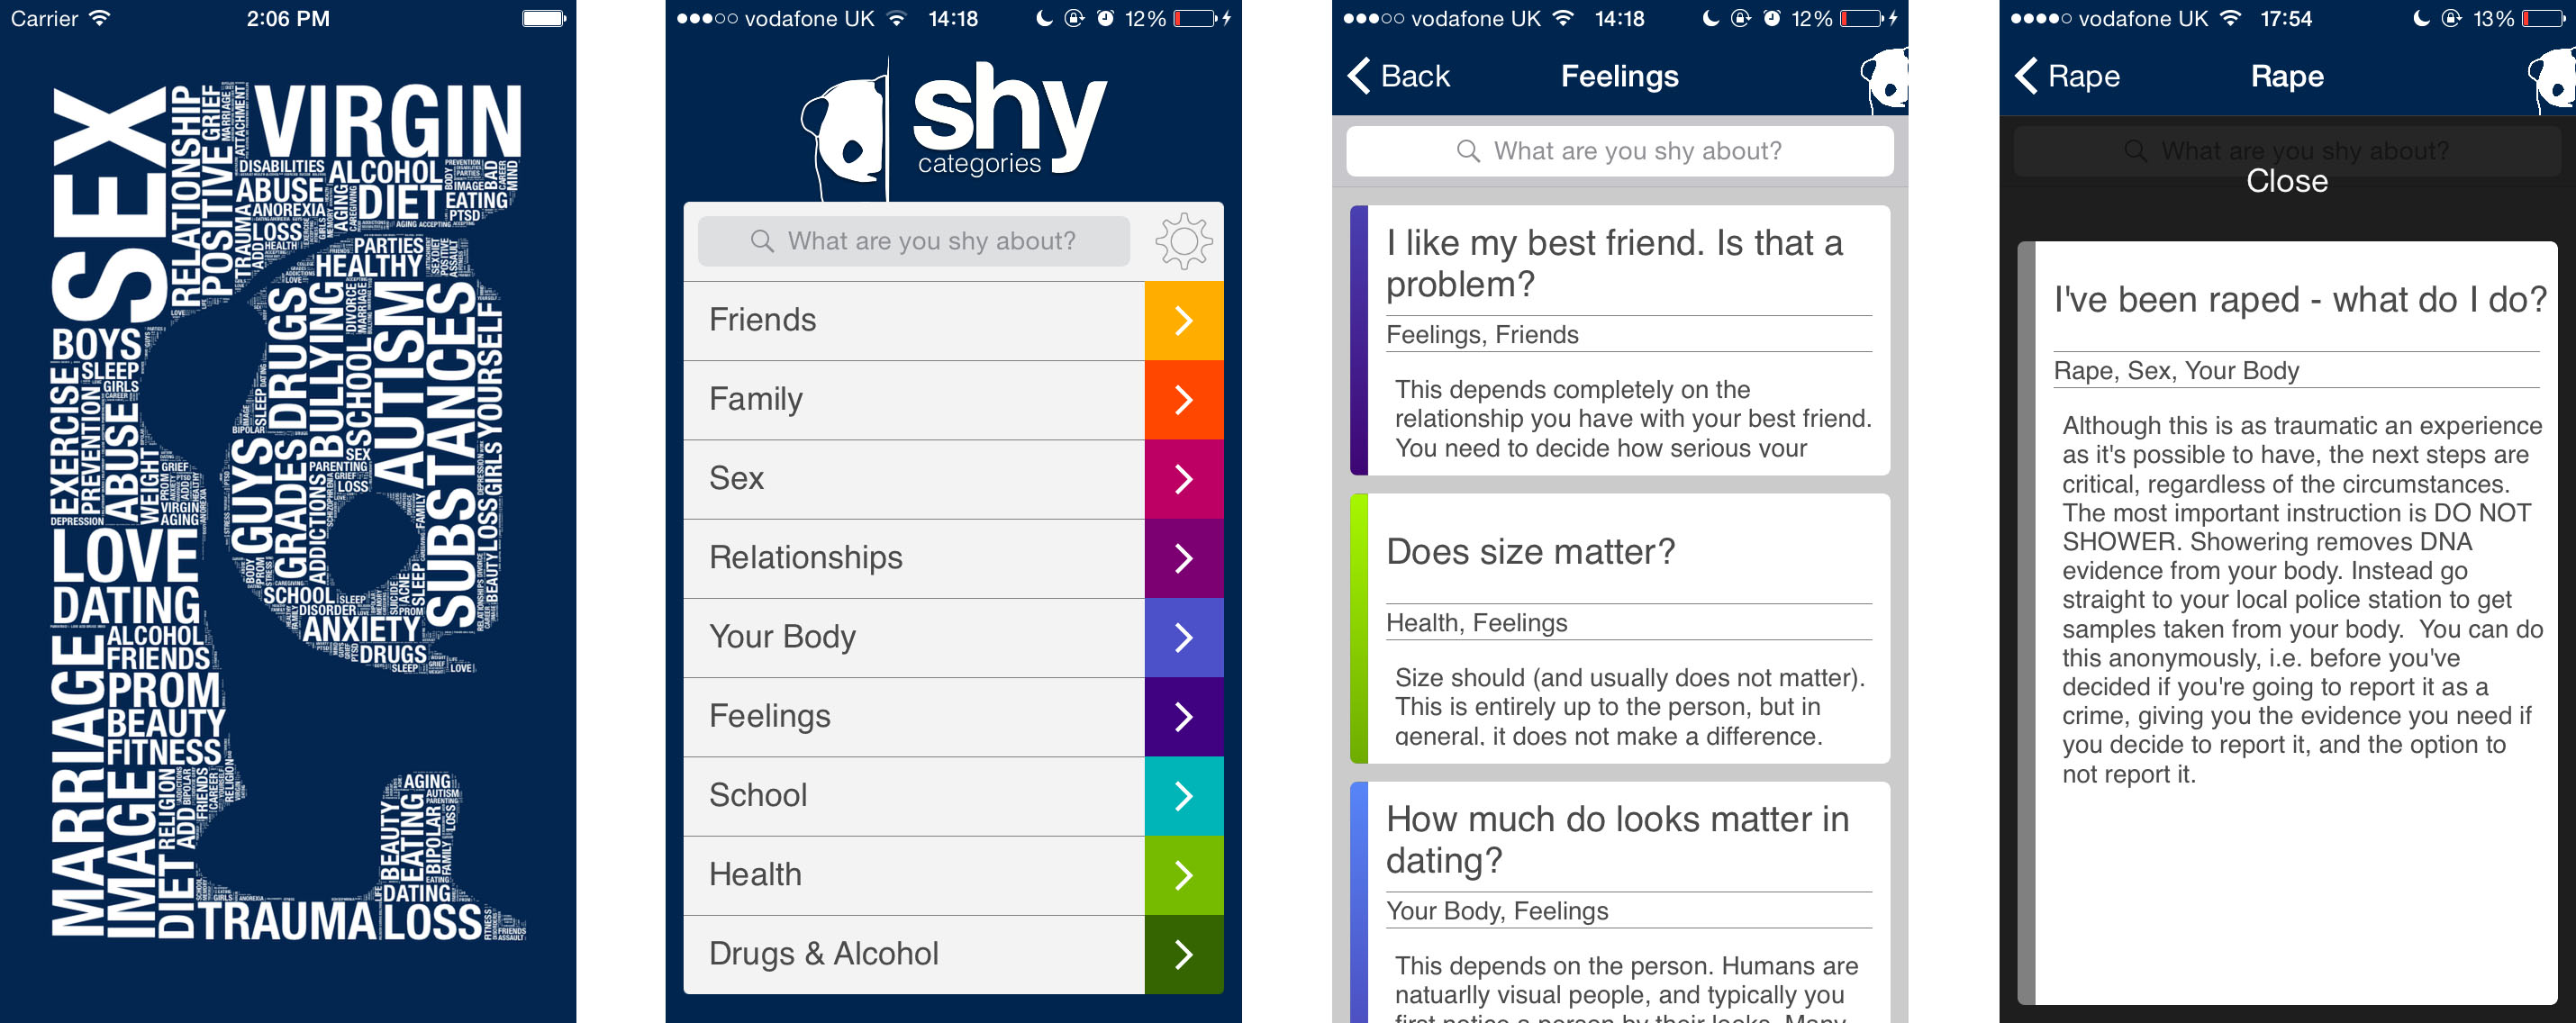
\includegraphics[width=\linewidth]{shy-screenshots}
\caption{Screenshots of Shy iOS App}
\label{fig:shy-ios-screenshots}
\end{figure}

\section{Motivation for this project}
Access to knowledge is a critical part of modern life.  It's also a Human Right, under Article 27 of the Universal Declaration of Human Rights~\cite{community1948universal}.  As members of a developed country, we have the facility to retrieve information and instantly communicate with each other using our smart phones, and commonly do it up to 200 times a day~\cite{falaki} which is a facility that hundreds of millions of individuals in developing countries live without.  This project aims to investigate the technical and ethical challenges behind this and to create a technology to give more people access to knowledge, and thus their human rights.

The project involves the use of a number of systems, including machine translation, an SMS input/output system and a system to build a profile on a user in order to facilitate high-quality targeted question-answer matching.  The system will also feature machine learning so that as time progresses, the quality of the answers it returns increases.  The use of these systems in one application along with complex ethics and privacy issues create an interesting project that draws together many technologies and discussions in a way that can be used as a basis for further research in the future.

\section{Aims of this project}
\label{sec:introAimsOfThisProject}

The first goal of this project is to assess and address the ethical issues that arise from the software that will be created.  These include the responsibility that the software and its developer has because of its position of trust to provide accurate information and to protect the privacy of its users by storing only necessary information, among others.  This project will do this by researching ethical issues relating to the technologies that the project will use, for example machine translation and user information storage.  This will then be used to feed the design process of the software and to specify the expected use-case of it.  Finally, the resulting software will be evaluated through experimentation, with volunteers asking the software a set of questions within a topic area, in a non-English language, and evaluate the relevance of answers returned.

Initially, the goal for this dissertation was to focus on questions relating to personal health, sex, relationships and family, which was as a direct result of the focus of 'Shy'.  Although a health and diseases database was located in the early stages of the project (Diseases Database, www.diseasesdatabase.com), it was targeted at professional uses for the data and came with a significant licence fee, as well as complex documentation that the provider customised specifically for each use-case.  An attempt was made to acquire a free academic research licence via email but this was unsuccessful.  Additionally, as the project progressed in the early stages it became clear that the author's original two-page document discussing ethical considerations with the project did not cover all possible situations.  Indeed, further significant ethical issues were still been discovered as far as eight weeks into the project, which would have required a complex ethics panel review, critically delaying this project.  One major issues was that any application that dispenses health related information that a user might act upon in a life changing manner has to always provide correct information in response to a query, since an incorrect response could lead to a user taking an action which leads to them harming themselves. No information source containing knowledge of a high enough quality with a licence that allowed it to be used in this project could be found. Another issue was that privacy, which is critical to a project in the area of personal health, couldn't be guaranteed since information would be transmitted in an unencrypted form via SMS.

As a result of the above issues with locating a reputable knowledge base and the complex ethical issues, a decision was made in early December 2014 to switch the target topic for questions to Geography and to use Wikipedia as a datasource, since it is openly available, well populated and multiple methods exist for extracting information from it.  In future work, it should be possible to extend this project to work with medical questions, if a high quality data-source is located and a solution to the ethical issues is found. A full discussion of possible future work is included in section \ref{sec:extending}.

\section{Structure of this report}
This report starts with a literature review in chapter~\ref{sec:literatureReview} where existing software, tools and services of a similar type to those that will be used in this project are presented, along with research into the ethical issues of the creation and use of the software under development. Comparisons between different software development life-cycles are also described and discussed.

Chapter~\ref{sec:method} describes the method that will be taken to develop the software and service.  This covers the software development life-cycle that will be followed, and sets out a plan for when development will take place.  Requirements will also be identified, described and categorised  as either functional or non-functional.  A method of evaluating the success of the software will also be discussed and chosen.

The design of the software, driven from information collected from the requirements, will be set out in Chapter~\ref{sec:design}.  The individual components that make up the technology will be described and discussed, followed by a set of annotated diagrams showing how these modules will interface with each other to build a complete system.  Finally, this section will include a description of the platform, language and other tools that will be used.

Chapter~\ref{sec:implementation} contains details about the implementation of the software.  This includes information on the tools that will be used to create components such as the SMS interface and question-answer matching system.

Results from the evaluation of the system will be presented in Chapter~\ref{sec:results}.  A discussion of these results and their implication on this project is then presented to the reader in Chapter~\ref{sec:discussion}.

Chapter~\ref{sec:evaluation} contains an evaluation of the software produced and the process taken to complete it.  Comparisons will be made to the success criteria, set out for the project in section \ref{sec:evaluatingSuccess}.

Thoughts on potential future research that builds on the work produced in this project are then displayed in chapter~\ref{sec:extending}.

Finally, the main achievements of this project are concluded in chapter~\ref{sec:conclusion} with closing thoughts.


% Lilian: This section should be expended, especially mentioning the consequences of such assumptions. Why do you make those assumption (e.g. time constraint, little or no consequences, ...). What limitation this may cause to your findings.  Shows a mastery of the field.
\section{Assumptions Within This Project}
This project will make the assumption that users of this service have basic literacy skills in \marginnote{Lilian: I no longer have language support, and you said to keep research in about it. Should I remove it from introduction / abstract etc?}a language supported by the project.  Although this is not a correct assumption world-wide, expanding the remit of this project to include a 'graphical' user interface that works over SMS would scale this project outside of the practical limitations of this project.

The main use-case for this project is going to be parts of the world with limited internet access.  Although these exist all over the world, the African continent is typical of this problem so I will focus my research in demonstrating a need for this tool there.

{\color{red} extend this}

\newpage

\chapter{Literature Review}
\label{sec:literatureReview}

{\bf The point of this is to show that I 'own' the material and subject (competence).  Show different points of view, choose a side, express a view on which I prefer and if I agree, critique.  Have objective goals.}

% TODO expand introduction to explain why sms, then look at related work in next section.  compare to smart phones loosely.
A significant amount of work has previously been undertaken in the area of making knowledge quickly accessible to us in the form of questions and answers.  To take one example, imagine that an individual needs to find the population of London as quickly as possible.  The initial step would be to search for information.  In the connected world, this is easy: a simple Google search returns the answers without even having to click through to any resources, as shown in Figure \ref{fig:googleInstant}.

\begin{figure}[htb] 
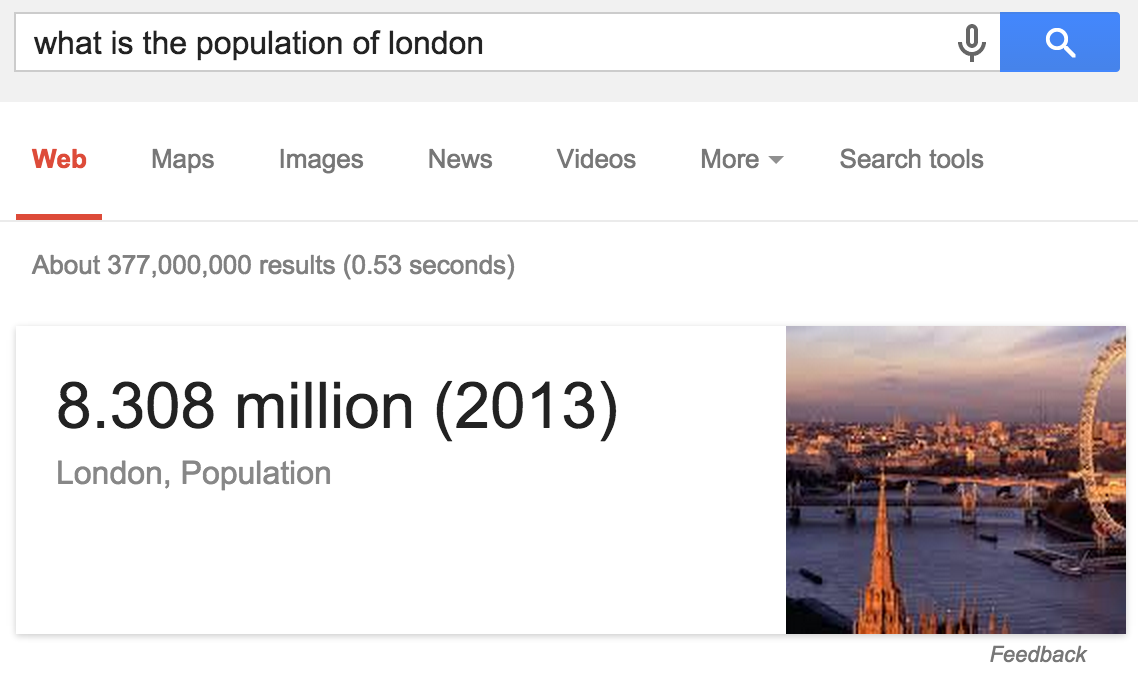
\includegraphics[width=\linewidth]{googleInstant}
\caption{Google Now information box.  Screenshot taken on 3rd February 2015.}
\label{fig:googleInstant}
\end{figure}

This is easy to do in the developed world where up to 75\% of the population are connected to the internet~\cite{ITU_Cell_Usage_2013}, with the population of elderly people been largely responsible for the remaining 25\%~\cite{Gov_Internet_Usage_UK_2014}.  This contrasts strongly with the situation in the African continent, where in 2013, internet usage had only reached 16\%~\cite{ITU_Cell_Usage_2013}, a figure largely inflated by South Africa where 5\% of the African population generate 2/3 of internet traffic from the African Continent~\cite{ITU_Cell_Usage_2013}.

% But there are other communication methods which are proven to work
\section{Previous work using SMS}
Although the above suggests that the African continent is majoritively disconnected, this is not the case.  Because of restrictions in the electricity available, the ways in which a non-smart phone can be used in Africa have far surpassed those in the developed world~\cite{Fox:2011:Online}, in part due to the longer battery life of a non-smart mobile phone compared to a smart mobile phone.  Interesting examples of SMS use in Africa include an automated service which sends an SMS to HIV/AIDS sufferers to remind them to take their medication, and a system for farmers that gives them the current market prices for goods, saving them from making regular long-distance trips to the market or relying on out-of-date information from a weekly radio broadcast~\cite{Aker_Mobile_Phones_2010}.

Interactive systems have also been developed to operate over SMS.  One successful example is mobile money platforms.  These allow for users from any background to pay and be paid for goods and to transfer money across long distances at negligible cost~\cite{Aker_Mobile_Phones_2010}.  One of the most highly adopted services is M-Pesa, which in Kenya alone was responsible for \textsterling5.7 Billion in transfers in 2012 \footnote{Data from Safaricom, M-Pesa operator in Kenya - actual value 817,085,000,000 Kenyan Shillings, converted to GBP on 1st November 2014 at rate of approximately 0.007.}.  M-Pesa gives users a balance linked to a national ID number from which they can pay for goods by sending an SMS with a cashier (recipient) number or pay outstanding bills in a similar way.  Non-subscribers can also use the system by depositing money with a M-Pesa cashier in exchange for an access code, which can be sent via SMS to a contact who can subsequently redeem it with their local cashier~\cite{Aker_Mobile_Phones_2010}.

This difference in standard use of mobile phones is demonstrated in the International Telecommunications Union's 2013 report~\cite{ITU_Cell_Usage_2013}, which shows that in Europe, for 790 million mobile subscriptions, 53\% of subscribers have mobile internet access (422 million), compared to 17\% in Africa (93 million have mobile broadband, out of 545 mobile subscribers).  This is due to the prohibitively high cost of accessing data services, regardless of the hardware that the user has.  In 2012 in Europe, 500 MB of data per month for 12 months cost 1.2\% of the average Gross National Income Per Capita (GNI pc).  In Africa, the average price was 30x this, at 36.2\% of an individuals GNI pc~\cite{ITU_Information_Society_2013}.

% No research has been undertaken investigating whether bringing knowledge through this method is viable option.

\section{Ethical Issues}
This project raises a number of ethical issues related to translation accuracy, providing information to people in an ethically acceptable way (with a focus on information accuracy) and maintaining user privacy.

\subsection{Ethics of Providing Information}
One significant issue for this project stems from providing information that may affect an individual or lead them to take a harmful action.

% TODO Finish Ethics of Providing Informatio

{\bf In a similar way to that which a teacher has a responsibility to teach accurate information to a pupil due to their position of trust, any service relied upon by a user must equally provide accurate information.  The result of not doing this could be providing inaccurate information that leads to a user carrying out an action that causes harm}.

% TODO Reword last two sentences.  This is something important and obvious - perhaps simple analogy is not necessary.  Perhaps give a generalised example.

% Lilian: You may want to look toward news paper (online/printed) to look at current/past issues that led to a law suit/inquiry and subsequent verdict/laws that may have been changed.

% Lilian: You should provide both point of view so do use this material, then you will have to critic both point of views. 
{\bf this needs to be waaaayyyyy expanded, but I struggled to find information that was useful.  There's lots on remote education, and on basic ethics of teaching, but I struggled to find anything specifically relating to ethics of ensuring information you provide is correct}.

\marginnote{teachers code of conduct, wikipedia ethics to provide infomration that contributos believe to be correct. doctors and gp's provide to the best of their knowledge}

\subsection{Ethics of Translation}
\label{subsec:ethicsOfTranslation}
A significant part of this project is represented by the support of multiple languages.  It is clear that translation on demand, at scale, needs to be automated by some kind of machine or algorithmic translation.

This project involves two blocks of translation.  These are:
\begin{itemize}
  \item The translation of the user's input into the language of the system (English)
  \item The translation of the answer to a user's question from the system language to their local language.
\end{itemize}
The latter of these raises some issues that do not apply to the former. To understand these issues it is first necessary to understand the two categories of machine translation.

Rule-based machine translation effectively treats human language in a similar style to programming languages.  Formal grammars and lexicons are used to represent words that exist in either the source or target language, structures representing the translation of individual words or groups of words.  Map structures contain mappings between individual or groups of words to their translated counterparts, sometimes with multiple results (a 1-to-many map), from which rules decide which is selected.  Maps and rule sets are created by trained computational linguists~\cite{kenny2011ethics}.

More commonly, Statistical Machine Translation (SMT) is used, for example, by Google and Microsoft in their translation products~\cite{kenny2011ethics, Google_Translate_Research}.  SMT learns mappings between strings of words of potentially unequal lengths from pre-existing original texts and their trusted human translations.  The accuracy and breadth of language support for translation increases as more source material is analysed by the system, as potentially erroneous or low quality translations can be identified and flagged.  SMT is also dependent on the quality of the human translation on the input material~\cite{kenny2011ethics}.

A significant issue that is present in statistical machine learning systems comes from the knowledge we assume an individual has and derives from a word; in this project, this affects the translation of the answers returned to a user.  In human translation this is solved by the translator's knowledge of the difference in material culture, allowing them to append necessary information to the resulting translation that the recipient might find useful.  In statistical machine learning, cultural awareness of material knowledge is a separate problem on its own.  {\bf formal reference to this, probably again from Kenny, but should be able to find better}.  To take one example from Melby (2006):

\blockquote{"when translating a French menu, a human translator might stop to think that an English speaker in France would appreciate being told that a steak tartare is served entirely raw, even if this information is not contained in the original text (because French people might be assumed to know this already). Such a translator would be aware of differences in material culture, and would be able to empathise with the English speaker who might choose to avoid the dish, given more information"~\cite{melby2006can, kenny2011ethics}}

This issue is a result of the translation engine not being capable of taking and using a complete representation of the expected cultural differences between those who speak the input language and those who speak the output language~\cite{melby2006can}. This does not apply to the first block of translation within the application where a user's input is translated into the language of the system, since the application will only need to parse text to identify geographical entities and the property been queried, making context unnecessary.

{\bf below should really be expanded and be in the discussion.  Explain the decision to keep translated answers in the database, which are pre-approved, to ensure no cultural misunderstandings.}

The potential uses of this system include distributing information that may be used by individuals making important decisions, regardless of whether that is within this project or in further work based off of this project, as cultural confusion such as this could have potentially catastrophic effects.

\subsection{User Privacy and Data Protection}
\label{subsubsec:userPrivacyAndDataProtection}
This project uses a simple Artificial Intelligence (AI) to keep a record of information that has already been returned to a user, to attempt to save sending repetitive information (saving the cost of additional SMS).  This raises another ethical issue though of privacy.  The material that a user has researched is likely to be sensitive; such is the nature of health related questions\marginnote{Lilian: Need to re-write this for new question subject, or can leave as a mark of the old subject topic?}.  This means that the information on a user has to be kept securely, in a way that an individual user can not be identified.

One way of doing this is using a technology called hashing.  Hashing is the technique of taking data as an input and generating an output value (called a 'hash') that is unique to an input.  Hash functions are ideally one way functions where given a piece of input data X, the output hash will always be a constant value Y, whenever and however the hashing algorithm is executed.  This allows a user's identifying information such as their phone number to be obscured, in such a way that the mobile number can not be recovered from the database.  When a question is received, the phone number (represented by variable X in the above example) can be hashed and the data for this number looked up from the database without the database application ever being aware of the phone number of the user.  In the example in Figure~\ref{fig:hashPhoneNumber}, a phone number (X) is used as input to an imaginary hashing function and the output hash (Y) is shown on the right hand side.  As just described, this number can then be used as the key for the user information database, shown in Table~\ref{table:hashDatabase} to retrieve the information needed for the AI.

{\bf reference the above from security engineering ross anderson, chapter 10 and 21?}

\begin{figure}[htb]
    \centering
    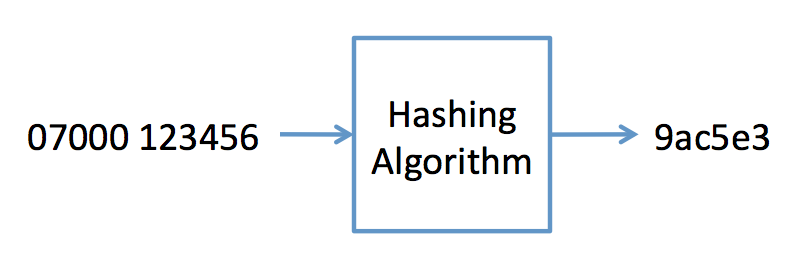
\includegraphics[width=200pt]{hashPhoneNumber}
    \caption{Hashing a phone number using an arbitrary hashing algorithm}
    \label{fig:hashPhoneNumber}
\end{figure}

\begin{table}
\begin{center}
    \begin{tabular}{| l | l |}
    \hline
    userId & userData \\ \hline
    8f64B2 & \{‘previousQuestions’:[13,301,170,577]\} \\ \hline
    9ac5e3 & \{‘previousQuestions’:[441,56]\} \\ \hline
    f9dd7e & \{‘previousQuestions’:[301,623,89,280,364,621,209]\} \\
    \hline
    \end{tabular}
    \caption{Example of software database: hashed phone numbers paired with a list of previous returned answer IDs. }
    \label{table:hashDatabase}
\end{center}
\end{table}

In practise it is possible for the output of a hashing algorithm not to be unique to a particular input.  This is known as the collision resistance property of a hashing algorithm and formally is the property of a hashing algorithm that determines the probability of the same output hash for two distinct random inputs~\cite{mitCryptographyMd5}.  It occurs because the range of possible input values is much larger than the range of output hashes, and because all valid inputs must map to an output there is repetition in outputs~\cite{mitCryptographyMd5}.  This property of hashing algorithms can be a security risk for some use-cases, where hashes are used to verify that data has not changed since been hashed.  In this case, a third-party may be attempting to generate alternative, malicious data with the same hash as some pre-existing data, to swap them undetected~\cite{securityEngineeringHashingAnderson}.  In the use-case of this project there is no security risk since hashes are only used to anonymise phone numbers; however a high collision resistance is necessary to ensure that two users of the system with distinct phone numbers don't get mapped to the same row in the database, resulting in poor quality question-answer matching or in the extreme worst case, privacy issues originating from returning to one user answers that are targeted to another.

Irreversibility is a necessary property of the hashing algorithm chosen for this project.  This ensures that the key used in the database cannot be used to retrieve the phone number of the user, thus protecting their identity.  Commonly used hashing algorithm families, such as the MD family (e.g. MD5) and SHA family are all designed to be one-way~\cite{schneierCryptanalysisMD5SHA}

\marginnote{Lilian: Is the wording of Bruce Schneier paragraph ok? Should I perhaps remove the last sentence?}
It should be noted that Bruce Schneier is a fellow at Harvard's Berkman center for internet and society.  He has been posting regularly for his newsletter and then blog since 1998 (over 16 years) and has published material related to this field throughout this time.  He has been involved in the creation of other cryptographic algorithms, such as the Skein hashing algorithm and blowfish block cipher, so may have a vested interest in discrediting other algorithms such as MD5 and SHA.  However, the essay cited above is written as a result of the Crypto 2004 Conference in California, where the algorithm that Schneier suggests should be used at the end is not one that he has involvement in.  For these reasons, his material should be treated as reliable.

Although hashing algorithms are computationally one-way, they can suffer from another type of vulnerability affecting the security of the original input data.  When hashes are used for short strings of information (passwords, for example), a simple way to try and retrieve the original data is to compute a dictionary of the hashes of lots of common passwords, from which matches can be found.  This idea has been extended to produce Precomputed Hash Chains and subsequently Rainbow Tables.  These are highly efficient data structures that consist of chains of processed input messages and their hashes with a reduce function to reach the next item in the chain, allowing original input data to be looked-up from its hash.  Both Precomputed Hash Chains and Rainbow Tables tend to be Terabytes in size, and as such they only exist in a significant form for the most commonly used hash functions (including MD5 and SHA)~\cite{Teat:2011:SCH:2016039.2016072}.  Within this project, this raises privacy implications, as hashes within the database would be 'convertible' to phone numbers.

In password authentication systems, this can be solved by the use of a technique called Salting~\cite{hashingPasswordsInfoSec}.  Salting is where a 'salt' - a piece of additional unique data - is added to each piece of input data before hashing, and then this salt is prepended to the output hash.  This nullifies the use of Precomputed Hash Chains and subsequently Rainbow Tables~\cite{hashingPasswordsInfoSec}. When checking if a plaintext password is equal to the hashed and salted representation, the salt from the stored hash is added to the plaintext password, the hashing algorithm applied and then the output compared to the stored obscured password. However, in this application this would prevent efficient lookup of users from phone numbers in the application, as the application would have to compare an input phone number against every user object in the database, which is computationally expensive and slow since a salted hash has to be computed for potentially every user record~\cite{hashingPasswordsInfoSec}.  

As such, it has been decided that the best way of protecting a user's phone number in the event of a database hack without significantly degrading performance is to salt phone numbers with a constant, large and complex salt. This means that a rainbow table would have to be specifically computed specifically for this application and would be extremely large in size.

\section{Software Design Life Cycles}
There are many software development life cycles that a developer or company has available to choose from.  Four common ones include the Waterfall Model~\cite{royce1970managing-FirstDescriptionOfWaterFallModelNotByName}, Iterative Model~\cite{briefHistoryOfIncrementalAndIterativeSoftwareDevelopment}\footnote{Iterative development came together from many concepts dating back to 1957.  There was no single paper that initially presented the entire concept, but this paper gives a summary of how the various concepts came together into the current Iterative Development model.}, Spiral Model~\cite{spiralModelSoftwareDevelopment} and the Agile Development Model~\cite{beck2001agile}\footnote{The Agile Manifesto brought together a group of Agile Methods which had been in use since the mid-1990's into a single concept, that of Agile Development.}. In order to choose which life cycle suits this project best, research into all four has been carried out.

\marginnote{Lilian: remove these two footnotes? Not always necessary to reference the original}

\subsection{The Waterfall Model}
The waterfall model consists of 5 phases of work, where each leads directly into the next.  It is a plan driven development model, which means that all process activities such as the implementation of the project must be planned and scheduled before work on them begins~\cite{Engineering}.  The five layers are shown in Figure \ref{fig:waterfallModel} and described below:
\begin{enumerate}
  \item {\bf Requirements}.  In this stage, both user and system requirements for the project are determined after examining the business goals for the project.  These form the system specification.
  \item {\bf Design}.  Here, a plan for the software development is created.  The overall architecture for the software is created, the external libraries to be used are chosen and the interaction between different modules is modelled.
  \item {\bf Implementation}.  In this stage, the software is implemented to match the design and architecture set out in the Design phase.  Unit tests are written to ensure that each module matches its specification.
  \item {\bf Testing}.  In this section the system is tested as a whole to check for any bugs that might not be picked up when testing individual modules in isolation.  The software is then delivered.
  \item {\bf Maintenance}.  Finally, the software is deployed and maintained.  This includes making changes to the requirements and subsequently the software implementation as the business goals change. ~\cite{sommervilleSoftwareEngineering}
\end{enumerate}

\begin{figure}[htb] 
\centering
    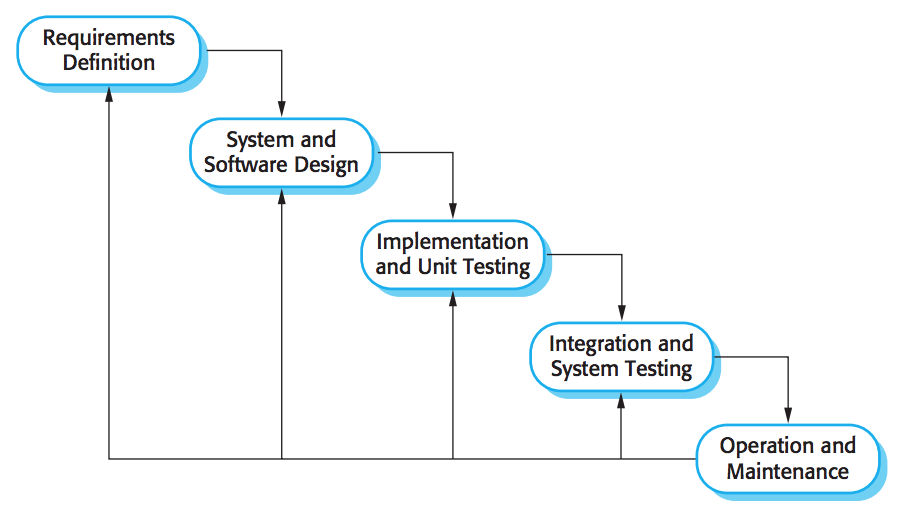
\includegraphics[width=0.8\linewidth]{waterfallModel}
\caption{Waterfall Development Model~\cite{sommervilleSoftwareEngineering}}
\label{fig:waterfallModel}
\end{figure}

A key advantage of the Waterfall Model is its simplicity: it is easy to understand and to use, saving time at the start of the project that would otherwise have been spent on learning and preparing to use a more complex model. The main disadvantage of the waterfall model is that once development has moved from one stage to another it cannot go back because the model is fixed and progresses in one direction only, until the maintenance step.

\subsection{The Iterative Model}
Iterative development is the practise of splitting the overall development of a project into multiple independent and distinct blocks.  A block contains a sequence of tasks which are essentially a mini life cycle, such that each iteration can really be thought of as its own project.  Each iteration tends to focus on a specific set of features such that when the iteration is complete the overall project is stable and the modules developed to date can be tested as a whole system~\cite{differenceBetweenLifeCycleModels}.

There are a multiple variations of the iterative development method. Two of these are Timeboxed Iterative Development where all iterations have a fixed duration, and Client-driven Iterative Development where each iteration contains the features that the client considers have the highest business value~\cite{larman2004agile}.

A common variation is based on the waterfall model as shown in Figure \ref{fig:iterativeDevelopment}.  The first three tasks in the cycle represent the first four stages in the waterfall model (Requirements, Design, Implementation and Testing), at which point there is the option to either evaluate progress so far and start another iteration, or to deploy the software and end development.  One significant difference between this and the waterfall model is that maintenance is not represented.

A key advantage of the Iterative Model is that it allows for the user to revise their requirements as they progress, making it dynamic and flexible which is ideal for small development teams.  This is also its disadvantage, in that the lack of fixed structure can be a weakness unless the project is planned well.

\begin{figure}[htb] 
\centering
    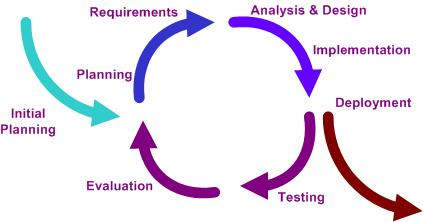
\includegraphics[width=0.8\linewidth]{iterativeDevelopment}
\caption{Iterative Development Method}
\small source: \url{https://commons.wikimedia.org/wiki/File:Iterative_development_model_V2.jpg}
\label{fig:iterativeDevelopment}
\end{figure}

\subsection{Boehm's Spiral Model}
The Spiral Model~\cite{spiralModelSoftwareDevelopment} was originally developed as a result of the adjustments that were commonly made to the waterfall model in large government projects.  The Spiral Model is a general model and can be used as a generator for other more specific models, given the parameters for a project such as its risks~\cite{boehm2000spiral}.  Models such as the waterfall model are specialisations of the spiral model~\cite{boehm2000spiral}.

In the Spiral Model each loop represents a stage of the software development, from planning on the inside loop to system testing and verification on the outside, as shown in Figure \ref{fig:spiralModel}. The cyclic nature of the model reflects the evolution of development of a software engineering project: the displacement from the origin shows an increase in the definition of the software, progress with the implementation and a decrease in the overall risk~\cite{boehm2000spiral}. With each spiral cycle in the model, stakeholder objectives are reviewed, risks identified and stakeholder approval and commitment sought before commencing the cycle~\cite{boehm2000spiral}.

\begin{figure}[htb] 
\centering
    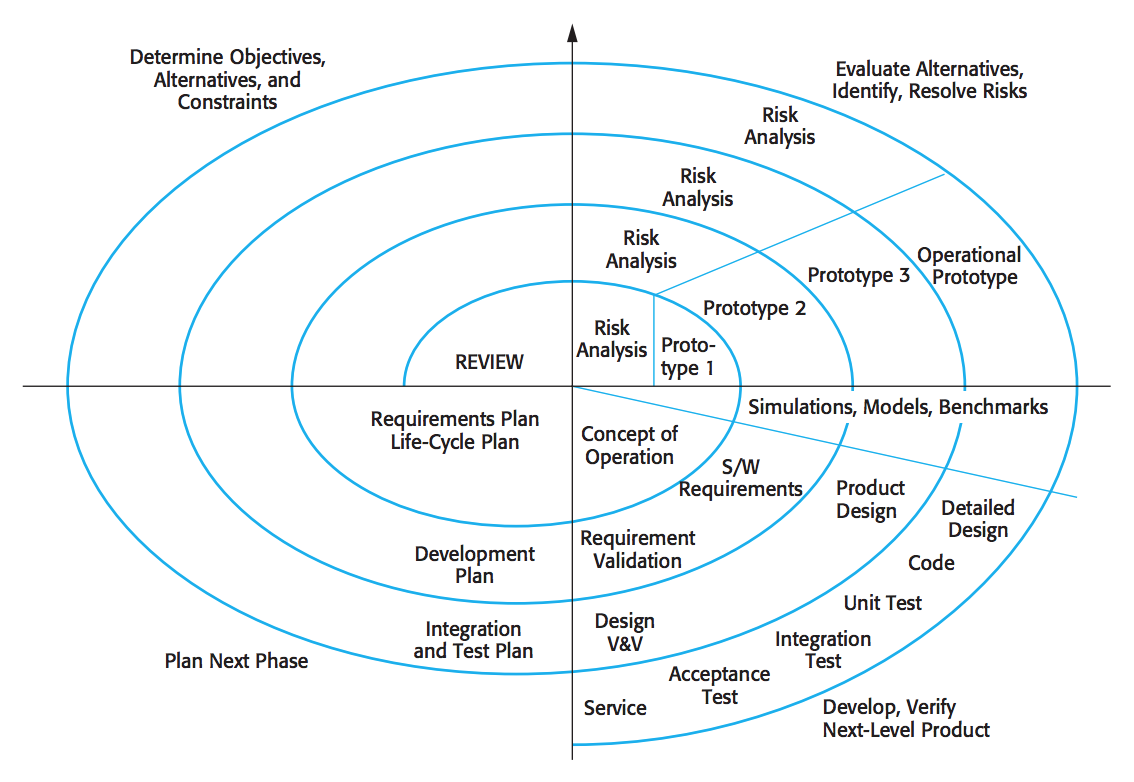
\includegraphics[width=0.8\linewidth]{spiralModel}
\caption{Boehm's Spiral Model~\cite{sommervilleSoftwareEngineering}}
\label{fig:spiralModel}
\end{figure}

A key advantage of the Spiral Model is the level of detail it models.  The stage of a sub-task within the entire development process is represented by the distance from the origin and each loop is split into small, well described sections. The main disadvantage is that the planning and use of the model is largely driven by the results of complex risk analysis on the sub-tasks~\cite{sommervilleSoftwareEngineering}.  Although this makes it favourable to large organisations, it has the opposite effect for smaller projects.

\subsection{Agile Development}
Agile Development essentially represents a group of development techniques targeted towards either the development of a small to medium sized product for sale or the development of a custom system within an organisation, where the customer has a high degree of involvement, for example 'Extreme Programming'~\cite{sommervilleSoftwareEngineering}.

Agile development is highly targeted towards teams with components such as Pair Programming, Collective Ownership, regular meetings and employee health (avoiding overtime) playing an integral part in the model~\cite{sommervilleSoftwareEngineering}.

\subsection{Development Life Cycle Summary}
\label{sec:developmentLifeCycleSummary}
Iterative development has been chosen as the model that this project will use, based on the following factors:
\begin{enumerate}
  \item Boehm's Spiral Model and Agile Development are both targeted towards development teams.  A significant part of these models relates to team interaction, so they are not appropriate to this project.
  \item The Waterfall Model is rigid and inflexible.  It does not allow for the changes to the requirements and implementation that might be proposed after evaluating the quality of the first implementation.
  \item The Iterative development model can be implemented effectively by a single developer, and supports the adjustment of requirements and implementation in each iteration of the cycle.
\end{enumerate}

\newpage
\chapter{Method and Requirements}
\label{sec:method}

In this chapter the method that will be followed for software development and an experimental evaluation of the software will be presented. The tools that will be used in the software will also be described.

\section{Plan for Software Development}
\label{sec:planForSoftwareDevelopment}
The Iterative Development Model was selected in Section \ref{sec:developmentLifeCycleSummary}.  Therefore, the development of this service will follow the principles set forth in this process. Software development will take place in stages representing each iteration of the iterative process.  After each iteration the software will be discussed in a meeting, with a focus on the developed capabilities, quality and any issues. Three iterations were scheduled that mapped to calendar months with the goal of having completed the software by the end of March.

Software development will begin in late December 2014 the first iteration is expected to be complete by the end of January which will demonstrate matching a variable directly by exact name to the Wikipedia API. A testing application will also be developed to aid development. The following additional iterations are planned, although it is expected they will evolve as the software changes and more clarity is achieved with regard to the goals.

During the second iteration running through February semantic analysis and matching of requested properties / keys in the data sources will be added to the application, and additional data sources will be researched and included.

In the final iteration running through March a natural language processing module will be constructed to handle questions in natural form as opposed to using a set syntax as had been used during development. Any additional tools needed to run an experimental evaluation of the software will also be developed.

In the initial specification of the project one aspect was to make the software developed capable of handling queries in multiple languages. However it has been decided after researching the issues of machine translation in section \ref{subsec:ethicsOfTranslation} that compatibility with multiple languages will be omitted from the software developed due to its complexity and the time constraints on this project. A discussion of how it can be added into the system in the future is provided in section \ref{sec:addingMultilanguageSupport}.

\section{Requirements}
\label{sec:requirements}
\subsection{Use Cases / User Goals}
Two personas were created to represent individuals who may have a need for the work resulting from this project, which can be seen in Appendix \ref{sec:appendixPersonas}. These are Nanjala, who is from Uganda, and Cedric, who is from Switzerland, and it is from these that user goals are extracted. These describe what a general user aims to achieve with this service.
\begin{enumerate}
  \item Nanjala wants to be able to read general information on any given topic.
  \item Cedric wants to be able to retrieve facts from direct questions.
  \item Both Nanjala and Cedric want to be able to achieve their goals entirely via SMS.
  \item Cedric needs a simple and efficient user interface that allows him to retrieve facts quickly. 
  \item Cedric wants to be able to feedback into the system when he finds an answer particularly useful or unhelpful. 
  \item Nanjala wants to be able to show the service to her friends without explaining how to use it every time.
  \item Cedric wants the system to protect his privacy, obscuring his identity.
  \item Nanjala wants to be able to ask questions as she would ask a friend without having to learn a syntax.
\end{enumerate}

\subsection{User Requirements}
\label{subsubsec:userRequirements}
User goals are distilled into formal user requirements.  Each user requirement corresponds directly to the correspondingly numbered user goal.
\begin{enumerate}
  \item Users must be able to request general or descriptive information on a geographical entity.
  \item \label{requirement:getFact} Users must be able to ask questions requesting a fact or statistic about an entity and get the answer or number they are looking for.
  \item Users must be able to interact with the system over SMS.
  \item Users must be able to make their queries and get responses quickly.
  \item Users must be able to feedback to the system when an answer is of noticeably low or high quality so the system can learn and improve.
  \item Users must be able to learn how to use the system themselves and this learning process should be quick.
  \item Users must be comfortable that their privacy is been protected whilst using the service.
  \item \label{requirement:userReqNaturalLanguage} Users must be able to interact with the system using natural language.
\end{enumerate}

\subsection{System Requirements - Functional}
\label{subsubsec:systemRequirementsFunctional}

System requirements are derived from the capabilities that the software needs to have to be able to support the user requirements. To support the user requirements in section \ref{subsubsec:userRequirements}, the application system must fulfil the following system requirements.

\begin{enumerate}
  \item \label{requirement:sysReqNaturalLanguage} The system will be capable of processing queries in natural language form.
  \item The system will receive queries via SMS, process them and then respond via SMS.
  \item The system shall use a datasource that contains both facts and descriptive text on geographical entities to answer queries.
  \item The system must be able to parse queries to identify the entity that is being asked about and the specific parameter of that entity that should be returned as the answer to the user's query.
  \item As well as giving direct facts and statistics, the system should be able to give general descriptive information on an entity.
  \item The system must be able to match words of similar meaning to the parameters in the data source.  For example, the word 'long' must be matched to the parameter 'length'.
  \item The system must learn from user feedback when answers that are returned are of high or low quality an apply this knowledge to future queries.
  \item The system must be self-explanatory, with the facility to offer instructions to a user.
  \item The system must use user state so that it can accept queries that are dependent on past questions, for example a query asking for more information or feedback on the quality of a past question.
  \item \label{requirement:easyToImplement} The system must be easy to implement and flexible, to accommodate future projects that make use of adaptations of this project.
  \item The system must obscure a user's phone number in the database.
\end{enumerate}

\subsection{System Requirements - Non-Functional}
\label{subsubsec:systemRequirementsNonFunctional}
Non-functional requirements are listed in table \ref{table:nonFunctionalRequirementsFitCrit} and are accompanied by a Fit Criterion, which will be used to identify whether a requirement has been met successfully.

\begin{table}
\begin{center}
    \begin{tabular}{| p{0.8cm} | p{6.0cm} | p{6.0cm} |}
    \hline
    ID & Non-Functional Requirement & Fit Criterion \\ \hline
    NF.1 & The system behind the SMS gateway must respond in a timely manner.  & From an SMS been received, a response must be sent within 20 seconds.  SMS transmission times on the cellular network and gateway are out of the control of this project, so are not accounted for. \\ \hline
    NF.2 & The answers returned must be of high quality.  & In testing, the system returns the correct information for at least 90\% of queries initially (before learning starts) if an answer is returned at all. \\ \hline
    NF.3 & Answers that are consistently rated poorly are are less likely to be returned. & In testing, after receiving a small number of negative ratings for an answer, a different answer is returned. \\ \hline
    NF.4 &Instructions to use the service should be clear and concise, with no ambiguity.  & In testing, having explained the purpose of the system, a user should be able to use the system with just the help information, without needing to ask for assistance. \\ \hline  
    NF.5 &The system should accept and be able to process questions in natural human language as opposed to a delimited message. & In testing, a user should be able to use the system for general questions without having had a syntax explained to them. \\ \hline
    \end{tabular}
    \caption{List of non-functional requirements and their Fit Criteria.}
    \label{table:nonFunctionalRequirementsFitCrit}
\end{center}
\end{table}

\section{Data Sources}
A number of possible datasources were identified from which data could be drawn from for this project.  These were all based off of Wikipedia (a large, linked source of knowledge), and include the Wikipedia API and various representations of the DBPedia Ontology.  In this section, both will be discussed and a decision will be made with regard to which ones will be used.

\subsection{Wikipedia API}
The Wikipedia API is a standard MediaWiki API and allows applications to query a page or resource for various parameters from a page, including the page contents, infobox parameters, citation list and links to other articles in various flat or multi-layered data structures~\cite{mediaWikiAPI}.  Interactions are made via a HTTP GET request to a URL containing the parameters, and responses can be received in JSON.  This makes the API easy to use and widely compatible, especially since JSON can be converted to a dictionary in most languages.

\subsection{DBPedia Ontology}
\label{subsec:dbpediaOntology}
The DBPedia Ontology is the result of a project that aims to build an OWL ontology representing all of the knowledge within Wikipedia.  The ontology has been manually created from the most commonly used infoboxes on Wikipedia and covers 685 classes with 2,795 properties, providing structured information on 4.2 million places, people, work, species and organisations~\cite{dbPediaIntro}.  This makes it especially good for use in applications since the data is both curated and well structured.

There are two ways of querying the DBPedia Ontology.  One is using the standard SPARQL ontology query software to make a query form the ontology structure; however this is complex as queries must be structured correctly and it is necessary to know the class structure of the entities being queried~\cite{dbPediaSparql}. Matching a question asked by a user to entities within the Ontology is difficult and outside of the time scope of this project.

In the event that the class structure is not known, queries can be made by querying the top-level representation of an entity in the ontology, which presents data in a similar format to that of the Wikipedia API, albeit in a 'cleaner' form (with human readable keys) as a result of the data been processed by hand.  Although the keys are of a more human-readable format, some material is abstracted within the ontology and so is inaccessible with a basic query.  An example of this is page for 'London' (accessible at: \texttt{http://dbpedia.org/page/London}), which does not have a parameter 'Mayor' with the value 'Boris Johnson'.  Instead it refers to a number of 'Leader Titles' and 'Leader Names', which include a reference to Boris Johnson

\subsection{Choosing the Source and Interface for this Project}
This project has a limited scope and time period available to it, and creating a system capable of identifying the relevant classes and then constructing SPARQL queries for looking up an abstract property is an example of an approach that is out of scope, as it involves natural language processing and semantic analysis of the names of the ontological classes, not just the query being made.  As such, this project will make use of a combination of the data from the Wikipedia API and DBPedia top-level entity representations, collecting keys from both and working with the key with the highest semantic relatedness match to identify the data-value that most likely is the answer to a user's question.  The DBPedia Ontology also provides access to the abstract at the same level as the infobox, so general descriptions of entities will be sourced from there.

\section{Processing Natural Language Queries}
Because of the nature of its audience, the system needs to be able to process input in natural language form rather than enforcing a formal grammar on users as described in User Requirement \ref{requirement:userReqNaturalLanguage} and System Requirement \ref{requirement:sysReqNaturalLanguage}. This involves constructing a natural language processing system to process queries and identify their meaning. In this project, queries are of a simple form: if a user is asking a question they are requesting a property of information about a given entity. An assumption is therefore made that each query consists of: a token representing the geographical entity been queried; a token representing the property been requested of that geographical entity; and some noise in the form of stop words.

\marginnote{Lilian: Ok to have this quite descriptive definition in the main text following straight on from the last paragraph?}
Stop words are words that are frequently used in in language but do not carry any significance themselves \cite{dataMiningStopWords}. It is common practise in Natural Language Processing to to remove these stop words before attempting to process an input \cite{dataMiningStopWords}. An example of a stop word is the word \texttt{the}.

It necessary to be able to identify the geographical entity in the query. This will be done using a Named Entity Extraction tool, of which there many available online including Cortical~\cite{serviceCorticalNex} and Dandelion~\cite{serviceDandelionNex}. These tools extract keywords from a text and in some cases are capable of categorising keywords according to an ontology. For example, Dandelion links entities to the DBPedia Ontology \cite{dandelionNex}.

The property about the geographical entity will be established by removing stop words, punctuation and the name of the geographical entity from the string.  In the input 'What is the height of the Eiffel Tower?', this would result in the string 'height'.

The result of this simple natural language processing should be that a sentence such as 'What is the Height of the Eiffel Tower?' is reduced to a structure indicating that the geographical entity is the 'Eiffel Tower' and the property is the 'height'.

\section{Evaluating Success - Experimental evaluation of the system}
\label{sec:evaluatingSuccess}
Success will be evaluated by establishing if the project fulfils its original requirements, based on the scenarios.  Many user requirements such as protecting the privacy of a user will be demonstrated through the software developed, whilst some that involve user interactions must be tested with users.  As such, user testing will be undertaken to evaluate three specific properties of the software through a trial usage and subsequent questionnaire: the usefulness and quality of the service, its usability, and the quality of the machine learning system.

Prior to running the experimental evaluation, a dry run will be undertaken with two participants. No data will be stored or collected - the purpose of the dry run is purely to establish early on any issues with the running of the experiment that would cause a problem during the real experiment.

\subsection{Client software for the experiment}
\label{subsec:clientSoftware}
The goal of this project has been to construct a piece of software that interfaces over SMS, as described in the project title. However there are practical limitations to running the experiment via SMS. During testing of the various services it was observed that HTTP-SMS Gateway Services added approximately a 5 second latency to both the sending and receiving of SMS, extending the length of time that a user would need to partake in the experiment to collect the same number of data points as could be collected when working straight over HTTP. In addition, the sending and receiving of SMS is costly and the savings made by not consuming SMS can be used to encourage participants to partake in the experiment. 

{\color{red} The interface is also an important consideration for the experimental evaluation - a key goal is to collect as many data points from participants as possible, whilst still maintaining some of the context in which the software will be used - on mobile devices. With regard to input speed, it is assumed\marginnote{reference?} that typing speeds are slower on mobile keyboards than full-sized physical keyboards, so data points can be collected more rapidly when working on a full-sized physical keyboard. In order to do this, a mobile app will be developed that interfaces with the software, and this will be run on a laptop with full-size keyboard. This gives participants use of a physical keyboard, allowing them to query the system more quickly and therefore making it acceptable to ask them to do a larger set of queries, and maintains the mobile context.}\marginnote{poor wording?}

\subsection{Questionnaire Design}
\label{subsec:questionnaire}
The questionnaire will aim to evaluate the usefulness of the system, the usability of the system and the quality of returned answers, and is based off of the IBM "Perceived Usefulness, Perceived Ease of Use, and User Acceptance of Information Technology" questionnaire~\cite{davis1989perceived}.  Questions were modified to suit the software being used in a situation without internet as opposed to a general workplace environment, and two questions were added: one to investigate the overall quality of answers returned to a user, and another to discover how trustworthy users felt the answers returned by the application were in general. 

Each question is formed by statement and a measure of how much the participant agrees with the statement. This is measured by selecting a value on a five-level Likert scale~\cite{likertScale}. The scale ranges from 1 through 5, where 1 is \texttt{strongly disagree} with the statement given, 3 is \texttt{neutral} and 5 is \texttt{strongly agree}.

A copy of the questionnaire that will be used is included in Appendix \ref{sec:appendixQuestionnaire}.

\subsection{Typical experiment plan}
\label{subsec:typicalExperiment}
At the start of the experiment, participants will be given both the consent form, included in Appendix \ref{sec:appendixConsentForm} and a document explaining what the software aims to achieve and what the participant should do, included in Appendix \ref{sec:appendixExperimentalInstructions}. The consent form sets out exactly what participants will be asked to do, the information that will be collected from them, and reminds them that they can withdraw at any time. The instruction sheet sets out some topic areas for the participant to research using the software, with a varying level of freedom within that topic. For example, they may be asked specifically to \texttt{identify the height of the Eiffel Tower}, or to identify a property of an entity of their choice such as \texttt{identify the population of a country of your choice}. Participants may also be asked to locate general information about a geographical entity. Constraints are placed on the area in which participants can query to limit the range of keywords used, thus focussing the machine learning onto a smaller group of words to allow a demonstratable improvement to be shown in the short space of this study.

After the experiment, participants will be asked to complete the questionnaire. Any additional comments arising during the post-experiment debriefing will also be noted beneath the questionnaire.

\subsection{Assessing success quantitively}
\label{subsec:assessingLearning}
As stated in section \ref{sec:evaluatingSuccess}, the experiment aims to evaluate three goals: the usefulness and quality of the service, its usability and the quality of the machine learning system. In the questionnaire, questions 1 through 6, 13 and 14 investigate the usefulness and quality of the system, whilst questions 7 through 12 investigate the usability of the system. Bearing in mind that this project is heavily constrained with regard to time due to constraints on the nature of it been a final-year project, it is not expected that the software will be as good as is possible. As such, the system's usefulness and usability will be deemed a success if it scores a significant positive average rating across all users in the questionnaire. The standard deviation of usefulness and usability ratings will also be inspected to judge whether users had a consistent experience or if different users had extremely different views on the software.

The machine leaning will be tested by inspecting the change in usefulness and quality rankings of the system made by users in the questionnaire as more participants use the system and provide ratings. The implementation of the machine learning system will be considered a success if a statistically significant positive trend is found in the usefulness and quality ratings when the ratings are sorted by the number of proceeding participants.

\newpage
\chapter{Design}
\label{sec:design}
In this section, the design of the system will be described, including information on: the structure of the server application and database; interactions with third-party services; systems used to protect user-identity; and the language, platform, tools and libraries used for development.

\section{System Design}
\label{sec:sysDesign}
In this section, the high-level design of the system software and its interactions with third-party services is described.  The system design was driven by requirements listed in sections \ref{subsubsec:userRequirements}, \ref{subsubsec:systemRequirementsFunctional} and \ref{subsubsec:systemRequirementsNonFunctional}, which were generalised to:

\begin{itemize}
    \item The system must be modular with points to add additional plugins, for example for additional data sources.
    \item The system must be easy to maintain, with distinct boundaries between functional components and behaviour.
    \item The database must be local to decrease the risk of exposing data.
    \item The system must have clear interfaces for interacting with the external world.
\end{itemize}

Based majoritively from these requirements, the requirements in sections \ref{subsubsec:userRequirements}, \ref{subsubsec:systemRequirementsFunctional} and \ref{subsubsec:systemRequirementsNonFunctional}, and the application of an informal gap-analysis between each iteration of the architecture, a modular system architecture was designed. This architecture details the modular structure of the application as well as some key pieces of functionality. A diagram showing the modular architecture is shown in Figure \ref{fig:systemArchitecture}, and shows that the main application contains 3 core modules: a module for performing semantic comparisons of text; a module for Natural Language Processing (NLP); and a module for extracting and processing information from sources. This final module contains two further sub-modules, one for fetching and processing data from each of the DBPedia and Wikipedia data sources. Key application functionality from the top level of the application is also shown including Query Parsing, where the type of the query is identified (for example, a question, a rating or a request for instructions) and Feedback Storage, where a feedback message is processed, linked to a previous question and stored in the database. In the NLP module the function for identifying the geographical entity been queried and the function for extracting the property a user is looking for from their question text are shown. Finally, in the Source Information Extractor and Processor module the function that applies past users feedback to answers to improve their quality is shown.

\begin{figure}[htb] 
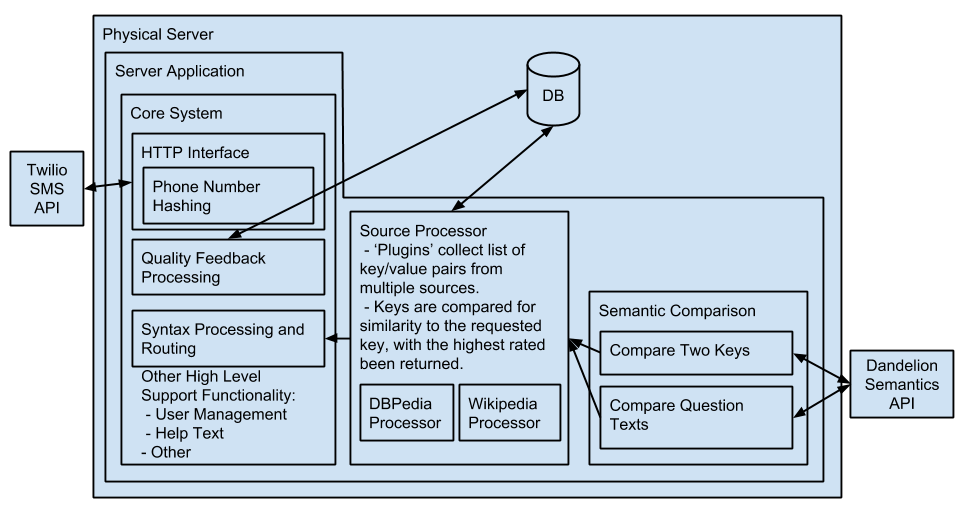
\includegraphics[width=\linewidth]{systemArchitecture}
\caption{ArchiMate diagram showing modular structure of the application relevant to computing the answer to a question.}
\label{fig:systemArchitecture}
\end{figure}

\subsection{Micro-system for Protecting User Identity}
\label{subsec:hashingUserId}

In section \ref{subsubsec:userPrivacyAndDataProtection}, the need to protect the privacy of a user and the general technique that will be used (involving irreversible hashing) are described.  The design of this system will now be discussed.

The main gateway into the system will be an HTTP call to a Python function called \texttt{sms()}, which takes the phone number of the user and the question being asked as its parameters.  This function represents a core part of the privacy protection system, by generating the hashed phone number and only using that when calling the function that computes the answer.  The user's unobscured phone number is only subsequently used when that function call has returned and it's time to send a reply SMS to the user. After that message has been sent the HTTP connection will close and the original number will be lost when the memory is released. As the computation of an answer only requires a general constant representation of user identity, not necessarily the user's real phone number, the specific value of the users phone number is not required within the computation of the answer.  As such, a hash is passed into the answer-computing function.  This hash will be used within the database to store a user's history and profile.  This means that only minimal user information (described in the physical data model in section \ref{subsubsec:physicalDatabaseDesign}) can be identified from the database, not the actual identity of a user.

\section{Language, Platform and Tools and Libraries}
\subsection{Language}
\label{section:designLanguage}
The language Python has been selected to be the main language in project for four reasons:
\begin{enumerate}
  \item Python is universally compatible and simple to execute.  Once the server application is written, it will be simple to migrate it between machines and adjust the application's configuration or environment.
  \item Python is commonly used and has significant community support in the form of libraries for all the tools that will be used in this project, for example libraries for querying common databases and for sending text messages.  This is useful as it will save time implementing common functionality like database calls.
  \item Python is an extremely flexible language in which it is easy to implement applications of this type without syntax issues.  This fulfils the system requirement in section (\ref{subsubsec:systemRequirementsFunctional}, point \ref{requirement:easyToImplement}) that the application is easy and quick to implement.
  \item The author has significant expertise in the language.
\end{enumerate}

A testing utility will also be created to query the application from a personal computer without using SMS.  A simple OS X Cocoa application will be created that queries the HTTP interface with JSON in the expected format and displays an answer.  Objective-C and and Mac OS X were chosen as the language and platform for this as the author has experience with Objective-C and uses a Mac.  There was no requirement for universal compatibility because the application is only for testing and development purposes.

\subsection{Platform}
The development platform of the utility will be Linux.  This is for three reasons:
\begin{enumerate}
  \item Linux manages Python and its libraries in a simple way without complex installers with tools like the Python Package Index (a library repository)~\cite{pypi}.
  \item Common libraries that will be used for creating a HTTP server, creating a REST API\marginnote{Lilian: should I explain what this is somewhere?}, making database queries and sending SMSs tend to be written primarily on the Linux platform.
  \item The author has familiarity with Linux and has access to significant Linux infrastructure under a grant from Rackspace.
\end{enumerate}

As previously stated, the interface to the application will be over the SMS platform.

\subsection{Database}
There are three tables of data that need to be stored.  These are the tables for: user profiles, to allow the application to handle queries that make use of 'state' with users; a list of keyword matchings between the requested property in the question asked and the property returned from the data source with quality ratings from user feedback, which the application uses to learn from and improve its answers; and a record of all asked questions, their answers and the ratings provided, to allow for questions to be answered based on highly rated previous answers.  

In the following section, the conceptual model is presented and then this is used to choose a database technology. Once the database technology has been chosen a logical data model and a physical database design are given.

\subsubsection{Conceptual Data Model}
There are four entities in the conceptual data model for this project.  These are:

\begin{itemize}
  \item {\bf Users:} An entity that represents a user. The user is identified via an obscured representation of their phone number.
  \item {\bf Last Question Asked by a User:} An entity containing the parameters of the last question.  This allows the system to handle stateful queries that are based upon a previous query.
  \item {\bf Keyword Pair Quality Ratings:} An entity that contains the property requested by a user, the property returned to that user, and the number of times a matching was ranked as being either one, two, three, four or five stars.
  \item {\bf Ranked Previous Answers:} A representation of a previously asked question, the answer text provided, and the rating given to the answer.
\end{itemize}

These entities are shown in the UML diagram in Figure \ref{fig:conceptualDatabaseDesignDiagram}, which also shows the entity relationships.

\begin{figure}[htb] 
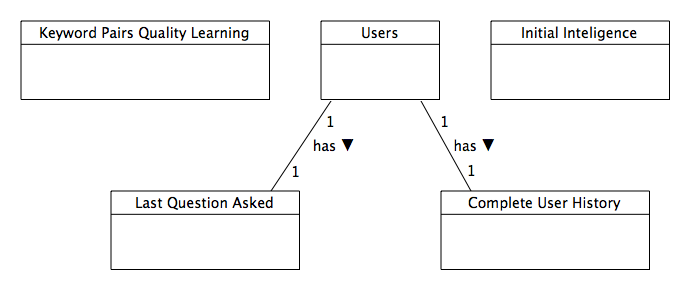
\includegraphics[width=\linewidth]{conceptualModel}
\caption{Conceptual Model of Data}
\label{fig:conceptualDatabaseDesignDiagram}
\end{figure}

\subsubsection{Database Technology}
\label{subsubsec:databaseTechnology}
The database technology requirements for this project are:

\begin{enumerate}
  \item The selected database must be as simple in implementation and interface with as possible, whilst still supporting the system requirements.  This is to allow for quick development and to avoid adding unnecessary complexity.
  \item The selected database must allow for storage and retrieval of records with multiple parameters.
  \item Support for records that are related to each other is not required, so relational databases are not needed, but not ruled out.
  \item The database must have a library for interfacing with it in the language of this project.
  \item The database should have built-in support for Sharding and Replication/Mirroring if possible to allow the application to scale. Sharding is the theory of distributing data and hence load across multiple servers~\cite{aboutSharding}, and replication is where data is stored on multiple machines to provide redundancy~\cite{aboutReplication}.
\end{enumerate}

There are a number of database technologies available that would fulfil the database requirements of this project.  Specifically, these can be split into two categories: relational databases and non-relational databases. Relational databases are used to store highly structured data in a table format~\cite{introToDatabaseSys}. Each table uses rows to represent a single record, and columns to represent the variables within that record~\cite{introToDatabaseSys}. These tables may contain constraints on the contained data to ensure integrity, such as limiting the range of a variable or enforcing that a variable may not be null~\cite{introToDatabaseSys}. Relational databases also encourage the use of table manipulation operations, where multiple tables are used to derive new tables with a processing stage in-between~\cite{introToDatabaseSys}. Relational databases also require a schema to be devised to formally structure the data~\cite{Parker:2013:CNM:2498328.2500047}.

Non-relational databases are specialised towards unstructured data, or where the data may be structured but there is a desire to not enforce a structure~\cite{Parker:2013:CNM:2498328.2500047}. Records are stored in collections which are similar to a table in a relational database, and collections then contain documents, which are similar to rows in a relational database~\cite{Parker:2013:CNM:2498328.2500047}. Unlike a relational database a collection does not have a set of columns or preset list of variables for each record~\cite{Parker:2013:CNM:2498328.2500047}. Instead, each record is a dictionary. Non-relational databases generally support storing relational data (entities that refer to other entities) by nesting documents inside of each other for one-to-one and one-to-many relationships~\cite{Parker:2013:CNM:2498328.2500047}. They also support referencing another document via its unique ID (which is assigned to all documents)~\cite{Parker:2013:CNM:2498328.2500047}. A downside of this latter technique is that the first object must be retrieved from the database to retrieve the ID of the referenced object before the referenced object can then be fetched in a relational-like query.

The two common databases used for each of these database categories are MySQL databases~\cite{mySqlDb} (relational) and MongoDB databases~\cite{mongoDb} (non-relational). In a Python application a MySQL database can be queried with an Object-relational mapping tool (ORM), which maps queries from the syntax of your programming language to a query in the SQL (a query language) and then maps the returned data to objects compatible with your programming language\footnote{ORMs also commonly apply optimisations to queries and validate them to ensure they are not malicious.}. MongoDB comes with a simple pre-existing client to query the database natively~\cite{libraryPyMongo}.

To fulfil the database requirements, the database chosen should be flexible with no fixed schema, querying should be easy in the Python language, and either support for relational queries or nested documents will be required. Additionally, it would be good if the database natively has sharing and replication/mirroring support so that in future work a stable and reliable system can be built. MongoDB meets all of these criteria, with no fixed schema, a simple method for querying the database, support for nesting documents and sharding and mirroring support for future expandability. In contrast, MySQL forces a fixed schema for data and requires a complex ORM for querying, although it does support relational queries natively and has support for sharding and mirroring~\cite{mySqlShardingReplication}. These properties of the two databases are shown in Table \ref{table:mysqlVsMongo}.

\begin{table}
\begin{center}
    \begin{tabular}{| p{4.0cm} | p{4.5cm} | p{4.0cm} |}
    \hline
     & MySQL & MongoDB \\ \hline
    Fixed Schema & Yes, reducing flexible & No, giving flexibility \\ \hline
    Querying Simplicity & Requires complex ORM and awareness of transactions, or construction of SQL queries. & Very simple with included MongoDB client. \\ \hline
    Records support nested parameters & No & Yes \\ \hline
    Supports relational queries natively & Yes & No \\ \hline
    Built in Sharding support & Yes & Yes \\ \hline
    Built in Mirroring support & Yes & Yes \\ \hline
    \end{tabular}
    \caption{MySQL \& SQLAlchemy vs MongoDB}
    \label{table:mysqlVsMongo}
\end{center}
\end{table}

From this comparison, the decision to use MongoDB has been taken because MongoDB has more flexibility than SQL meaning that development will be less time consuming, and writing queries is easier in Python with the built-in MongoDB Library~\cite{libraryPyMongo}.

\subsubsection{Logical Database Design}
Having decided that the database technology will be MongoDB which supports nesting in section \ref{subsubsec:databaseTechnology}, the logical design of the database is able to reduce the number of entities from four in the conceptual model to three.  This is because there is a one-to-one relationship between the \texttt{User} and \texttt{Last Question Asked by a User} entities, so the \texttt{Last Question Asked by a User} entity can be nested inside of the \texttt{User} entity as it only contains a small number of user-specific fields.  This will simplify the implementation, meaning that a smaller number of collections will be needed to contain the entities.

The logical database requirements are listed in Table \ref{table:logicalDatabaseDesignListing} and represented graphically in Figure \ref{fig:logicalDatabaseDesignDiagram}.

\begin{table}
\begin{center}
    \begin{tabular}{| l | p{6cm} |}
    \hline
    Table/Collection & Parameters \\ \hline
    Users & (\underline{id}, cellNumber, history, (lastQuestionText, lastQuestionRequestedProperty, lastQuestionReturnedProperty)) \\ \hline
    KeywordPairingRatings & (\underline{id}, givenProperty, returnedProperty, oneStarRatings, twoStarRatings, threeStarRatings, fourStarRatings, fiveStarRatings) \\ \hline
    RankedPreviousAnswers & (\underline{id}, question, answer, rating) \\ \hline
    \end{tabular}
    \caption{Logical Database Design.  Underlined fields represent primary keys.}
    \label{table:logicalDatabaseDesignListing}
\end{center}
\end{table}

\begin{figure}[htb] 
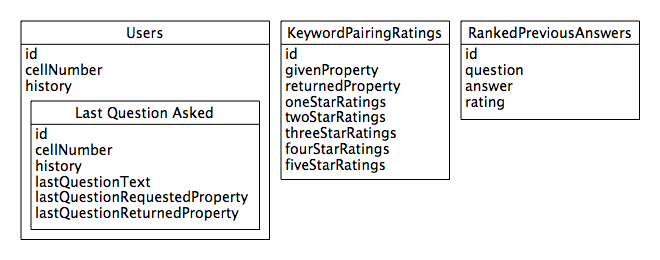
\includegraphics[width=\linewidth]{logicalModel}
\caption{Logical Model of Data}
\label{fig:logicalDatabaseDesignDiagram}
\end{figure}

\subsubsection{Physical Database Design}
\label{subsubsec:physicalDatabaseDesign}
As previously discussed section \ref{subsubsec:databaseTechnology }, MongoDB separates groups or types of entity into collections (which are similar to a Table in an SQL database) but does not place restrictions on the structure of objects within a collection.  The general structure of each document in a collection for this application is shown in Table \ref{table:collectionStructure}. A small change was made between the logical and the physical database designs with the storage of ratings in KeywordPairingRatings. In the logical model these were individual counts of ratings at the five different levels (for example, a count of one-star ratings, a count of five-star ratings, etc) however in the physical model this was converted to a list of ratings received (e.g. \texttt{[5,5,3,4,5]}). This made the implementation more compact as five different variables did not need to be addressed every time the ratings were read or written to.

The database software MongoDB will be hosted on the same server as the main application, as shown in Figure \ref{fig:physicalServerDb}.

\begin{figure}[htb] 
\centerline{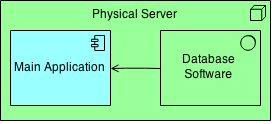
\includegraphics[width=0.6\linewidth]{physicalServerDb}}
\caption{ArchiMate diagram showing the structure of the main server, which runs the application and hosts the database.}
\label{fig:physicalServerDb}
\end{figure}


\begin{table}
\begin{center}
    \begin{tabular}{| l | l |}
    \hline
    
    Users &
    \begin{lstlisting}
    {
    '_id',
    'cellNumber',
    'history',
    'lastQuestion' : {
        'text',
        'givenProperty',
        'returnedProperty'
        }
    }
    \end{lstlisting}
    \\ \hline
    
    KeywordPairingRatings &
    \begin{lstlisting}
    {
    '_id',
    'givenProperty',
    'returnedProperty',
    'ratings'
    }
    \end{lstlisting}
    \\ \hline
    
    RankedPreviousAnswers &
    \begin{lstlisting}
    {
    '_id',
    'question',
    'answer',
    'rating'
    }
    \end{lstlisting}
    \\ \hline
    
    \end{tabular}
    \caption{Typical Document in each MongoDB Collection}
    \label{table:collectionStructure}
\end{center}
\end{table}

\subsection{Libraries}
In this section the libraries that were used in the server application in this project are presented. These include the libraries for querying the database, creating an HTTP server and sending SMS.

\subsubsection{Database Querying}
MongoDB comes with a Python client called PyMongo~\cite{libraryPyMongo}, which is developed by the same developers as MongoDB.  It is the recommended tool to interact with a MongoDB database~\cite{pyMongoDoc} and has good community support, so it will be used in this project.

\subsubsection{Creating HTTP Server and REST API}
The application needs to have an HTTP interface to allow interactions with it via SMS.  As a result of the non-functional requirement "The system behind the SMS gateway must respond in a timely manner" in section \ref{subsubsec:systemRequirementsNonFunctional}, the application will need to be able to process multiple HTTP requests concurrently to prevent requests queueing up and responses been significantly delayed.

To create an HTTP Interface, the latest Web Server Gateway Interface (WSGI) specification (version 1.0.1, published as PEP 3333)~\cite{eby2010python} will be followed as it is the industry standard. The WSGI specification describes a general interface between web servers and web applications or frameworks (such as Twilio) in the Python language, thus describing how the web server should be constructed.

In this project, two tools are needed: a WSGI server, and a framework for writing WSGI applications. Flask will be used for the framework as the author has extensive experience using it and it is compliant with the WSGI standard~\cite{libraryFlask}.

With respect to the WSGI server, many implementations exist such as a simple WSGI server included in Flask~\cite{libraryFlask} called Werkzeug~\cite{libraryWerkzeug}, and the Gevent WSGI server~\cite{libraryGevent}.  Support for multiple concurrent HTTP connections is not a requirement in the WSGI specification, and so some WSGI servers such as the implementation of Werkzeug in Flask do not support this even though Werkzeug does natively support processing multiple HTTP requests concurrently. It does this by specifically enabling threading and increasing the default maximum number of processes from one~\cite{werkzeugThreading}. The implementation of Werkzeug in Flask has these disabled in the source code because Flask uses thread-local storage (memory that is local to a single thread) and so cannot support concurrent HTTP requests on new threads~\cite{flaskThreading}.

A library called Gevent will be used to replace Werkzeug in Flask as it does support concurrent HTTP connections~\cite{geventImplementingServers} using using the Greenlet library~\cite{libraryGreenlet}, which provides a notion of micro-threading (coroutines). When a new HTTP request is received, Gevent creates a new Greenlet, thus preventing the main thread been blocked and allowing multiple concurrent HTTP requests. The creation of the Greenlet is described in the preceding reference(\cite{geventImplementingServers}). 

\subsubsection{Sending SMS}
There are a number of SMS providers with HTTP gateways available to choose from, all of which are similar. For this project, the provider must match the following criteria:
\begin{itemize}
  \item Forwards received messages to a REST API to enable easy development.
  \item Supports sending messages via a REST API which also enables easy development.
  \item Has good coverage of countries so that users from many countries can use the service.
  \item Has a 'good' reputation. This is because user privacy is still an issue, since data is unencrypted when been sent over SMS, so the provider should be trustworthy.
\end{itemize}

It is difficult to measure the reputation of a provider accurately, but one possible way of doing this is by looking at the number of significant clients they have.

Two services considered were that matched these criteria.  These were Twilio~\cite{serviceTwilio} and Plivo~\cite{servicePlivo}. Both use REST APIs for handling incoming messages and for sending responses. Both Twilio and Plivo have comparable coverage as well: Twilio state that they send and receive SMS with numbers in 198 countries~\cite{twilioCoverage}, and Plivo state that they support 207 countries~\cite{plivoCoverage}\marginnote{Lilian: remove footnotes about bias? Also, ok to mention a RAW URL?}\footnote{This is referenced on a marketing page (https://www.plivo.com/twilio-alternative/) where Plivo compare their product to Twilio's, so is likely to be biased}. The difference is trivial, as the number of recognised independent states in the world is between 190 and 200 depending on listing; the US Government recognises 195~\cite{usStateDepartmentListOfIndependentStates}.

With regard to reputation, for this project it was decided that Twilio is preferable to Plivo. Although it is difficult to measure reputation accurately, Twilio was founded in 2007 and has an group of clients including PayPal, Uber, Sprint and Airbnb, compared to Plivo, which was founded more recently in 2011.

\subsubsection{Semantic Analysis - Measuring semantic relatedness between texts}
\label{sec:choosingSemanticAnalysisApi}
Semantic comparison of text will be used for two purposes within the project: to match keywords from datasources, for example, if a user asks \texttt{how tall} something is, the property \texttt{height} would be appropriate to return; and to match questions with identical meaning to each other to save the application doing a full analysis of the data sources again. The requirements for these use-cases are different: for the former the tool needs to compare pairs of either single words of short strings or words for semantic similiarity; and for the latter the tool needs to be able to compare full sentences for semantic similarity.

Semantic similarity is a measure of how semantically alike entities are in their meaning, for example, \texttt{bank} and \texttt{trust company}~\cite{Budanitsky:2006:EWM:1168106.1168108}. A more general measure exists called Semantic Relatedness. Whereas semantic similarity compares entities by their meaning, entities may be semantically related by additional lexical relationships such as antonymy (the opposite of an entity, for example, \texttt{tall} and \texttt{short}) and meronymy (entities that are a part of another entity, for example, \texttt{car} and \texttt{wheel})~\cite{Budanitsky:2006:EWM:1168106.1168108, budanitsky2001semantic}. Both use-cases in this application will be using semantic similarity as semantic relatedness is too general. An example using the datasource keyword matching usecase is that using semantic relatedness, the word \texttt{tall} would be related to \texttt{width} as well as the target word of \texttt{height} as a result of antonymy, potentially cluttering results. In the second use-case, consider a highly rated question in the database of \texttt{What is the population of England?} and then the question of \texttt{What is the population of London?} being processed. London is a part of England, so there is the potential for the population of England to be returned instead of the population of London.

A key requirement for the algorithm and method used to compute semantic similarity is that it can be implemented in compliance with the system requirement in section \ref{subsubsec:systemRequirementsFunctional}, point \ref{requirement:easyToImplement}, that the system is easy to implement. A number of algorithms were discovered for calculating semantic similarity based on the WordNet lexical database~\cite{wordNet}, such as the Leacock-Chodorow and Resnik algorithms. Although mathematical representations of these algorithms are published~\cite{leacock1998combining,resnik1995using}, to fulfil the aforementioned requirement a pre-implemented semantic comparison tool is needed as implementation of these algorithms would be a non-trivial software engineering project. Both of the Leacock-Chodorow and Resnik algorithms are available in a Perl package as part of WordNet::Similarity, a set of Perl modules with an optional web interface for integration into applications. No other open-source libraries were found, so during application design, an attempt was made to use the WordNet::Similarity tools by calling the Perl scripts from Python code. This proved complex as there were numerous out of date dependencies to trace and install.

An alternative to using a specific algorithm in a library was to use an online semantics package. Two were identified: the Cortical Compare API~\cite{serviceCorticalSim}; and the Dandelion Similarity API~\cite{serviceDandelionSim}. Both take two pieces of text and return a value representing the semantic similarity of the texts. The Cortical API was found to be better suited for comparing single word or short multi-word terms using its \texttt{term} type~\cite{serviceCorticalSim}, often returning errors when queried with two texts with a similar syntax, and in contrast the Dandelion API is better suited to single or multi-sentence blocks of text~\cite{dandelionSim}.

Both the Cortical and Dandelion APIs interface via a HTTP REST interface, so will be simple to implement. They are also in active development with support teams. For these reasons, they have been selected to be the semantic comparison tools used in this project.

\subsubsection{Semantic Analysis - Discovering Named Entities in text}
\label{sec:choosingNamedEntityExtractionApi}

A named entity extraction tool is required to establish the geographical entity ('place') in a users' question. The requirements of the tool were:
\begin{enumerate}
  \item Accepts a string of text and returns a list of keywords representing the place.
  \item \label{nexRequirement:categoriseKeyword} Keywords are categorised by a group classes, allowing for differentiation between a keyword representing a place, concept or person.
  \item Accessible via a HTTP REST API for ease of implementation (fulfilling functional system requirement \ref{requirement:easyToImplement} in section \ref{subsubsec:systemRequirementsFunctional}).
\end{enumerate}

During initial research, two keyword extraction APIs were discovered: the Cortical Keyword Extraction API~\cite{serviceCorticalNex} and the Dandelion Named Entity Extraction API~\cite{serviceDandelionNex}. However, the Cortical API does not fulfill requirement \ref{nexRequirement:categoriseKeyword}, simply returning a list of keywords. In comparison the Dandelion API returns a complex data structure which includes a list of DBPedia classes that the keyword is an instance of.

Research was done to identify a way of using the Cortical API to extract keywords and subsequently categorise the keywords after they have been been identified; however as there was no significant benefit of the Cortical API over the Dandelion API this was discounted and the Dandelion API chosen.

Results from the Dandelion API were checked against the \texttt{Place} class in the DBPedia Ontology by checking their \texttt{types} list (a list of DBPedia classes that the keyword fits into) for the string \texttt{http://dbpedia.org/ontology/Place}.

\newpage
\chapter{Implementation}
\label{sec:implementation}
This section will describe the implementation of the server application and the clients developed for testing and evaluation. In the server application focus will be given to the tools and services used, the natural language processing system, the method used to identify answers and the machine learning aspects of the application.

Code used within this project and discussed in this section is located in the following Git repositories:
\begin{itemize}
  \item \texttt{https://github.com/samheather/dissertationServer} - This repository contains the code for the server application.
  \item \texttt{https://github.com/samheather/dissertationClient} - This repository contains the Xcode Project and code for the Mac OS X testing client, used in development of the application.
  \item \texttt{https://github.com/samheather/dissertationIos} - This repository contains the Xcode Project and code for the iOS client application, used in the experimental evaluation of the application. It has been constructed for an iPhone 5 screen size.
\end{itemize}

\section{Implementation Overview}
As discussed in section \ref{sec:developmentLifeCycleSummary}, the implementation was completed whilst following the iterative development process. Software development took places in stages which represented each iteration, and after each iteration a version of the software was demonstrated in a weekly meeting. In these meetings, the software's capabilities and success rate were discussed, and requirements were re-evaluated based on progress. Ideas for expansions to the software (for example, the Natural Language Processing, which was not in the original plan) were also discussed.

The software has been constructed in a modular manner to allow easy future expansion and modification. This modular structure is described in section \ref{sec:sysDesign}, where the system design is presented.

\section{Tools and services used}
\label{sec:toolsAndServices}
The following tools and services were used in the implementation. These were chosen to fulfil the requirements detailed in section \ref{sec:method}.
\begin{itemize}
  \item Python was the programming language used in this project. This was due to a number of reasons, including that the author had experience with writing an application with some similar characteristics as those in this project.
  \item MongoDB version 2.6.6 was used as the database software in this project.
  \item Both the application server and the database server were hosted on an Ubuntu version 14.10 "2 GB General Purpose v1" Linux server, hosted by Rackspace in London.
  \item No integrated development environment (IDE) was used in the development of the server application. The author chose to use textural editors due to familiarity with them, and it was felt that the assistance provided by an IDE with managing modularity/abstraction/semantic checking would not be of significant benefit, bearing in mind the size of the server application.
  \item An IDE was used in the development of the client applicatios to reduce the use of expensive SMS during testing. This was written in Objective-C for Mac and iOS, and created in the Xcode IDE, which is the industry standard.
  \item The Twilio SMS Service~\cite{serviceTwilio} was used to facilitate the SMS interface to the server application.
  \item The Cortical~\cite{serviceCorticalSim} and Dandelion~\cite{serviceDandelionSim, serviceDandelionNex} APIs were used for semantic analysis of text.
\end{itemize}

In addition, the following Python libraries from the Python Package Index~\cite{pypi} were used within the server application:
\begin{enumerate}
    \item Greenlet~\cite{libraryGreenlet} - provides a notion of micro-threading (coroutines), which allows the server to process multiple HTTP requests concurrently.
    \item gevent~\cite{libraryGevent} \label{librariesUsed:gevent} - a coroutine based networking library for Python. gevent provides a Web Server Gateway Interface (WSGI) server that supports processing multiple requests concurrently, using Greenlet.
    \item PyMongo~\cite{libraryPyMongo} - Python library containing tools to work with MongoDB databases.
    \item ujson~\cite{libraryUjson} - Twilio uses JSON as the format for HTTP requests, so it makes sense to use it for all requests. ujson allows for effecient encoding and decoding of json to and from Python data structures.
    \item Twilio~\cite{libraryTwilio} - Twilio library used for receiving and sending SMS.
    \item lxml~\cite{libraryLxml} - Used in the 'Wikipedia Utils' library, which handles interactions with the Wikipedia API. lxml is used for processing XML/HTML in Python.
    \item Flask~\cite{libraryFlask} - a micro-framework for web applications, used for its simple syntax for defining HTTP routes (URLs that trigger Python functions). Flask also comes with a WSGI server, but it does not support processing multiple HTTP requests concurrently, so it is replaced with the Gevent WSGI server in point \ref{librariesUsed:gevent}.
    \item NumPy~\cite{libraryNumPy} - Numerical Python (NumPy) is used for outlier detection in the rating system. It provides a function call for calculating the standard deviation of a set of numbers.
    \item re - a Regular Expression matching library built into Python which is used in the 'Wikipedia Utils' library and in application code for converting CamelCase text to Snake case text.
    \item Wikipedia Utils~\cite{libraryWikipediaUtils} - a library used for abstracting the Wikipedia API.
\end{enumerate}


\section{Implementation of SMS interface}
The SMS interface to the application was developed using the Twilio SMS service and Library~\cite{serviceTwilio, libraryTwilio}. A HTTP interface to the application was hosted using Flask~\cite{libraryFlask} at \texttt{<server\_url>/sms}, and the Twilio service was configured to make a request to this URL when an SMS was received. The function \texttt{sms()} is executed upon receiving a request on the \texttt{<server\_url>/sms} address, which extracts the phone number of the user and the text of their message from the request. The number is obscured, as explained in section \ref{subsec:hashingUserId}, and then the function \texttt{start()} is called with both the obscured number and the text from the message. This function then computes the answer to return to the user, described in section \ref{sec:implementationOfAnswerLocationSys}, and the response is sent back to the user using the Twilio library to make a HTTP call to the Twilio service.

The service provided by the application and its service are shown in the ArchiMate diagram in Figure \ref{fig:systemSmsInterface}.

\begin{figure}[htb] 
\centerline{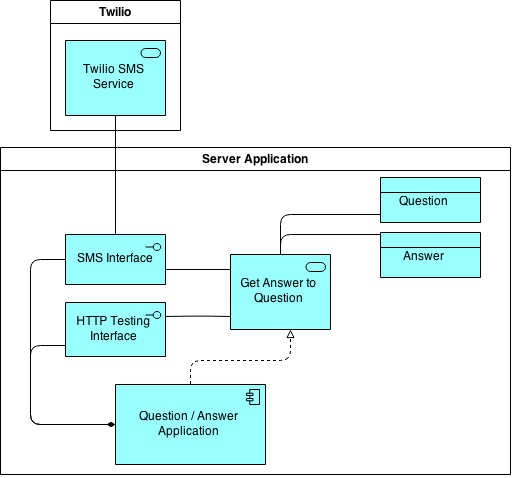
\includegraphics[width=0.8\linewidth]{systemSmsInterface}}
\caption{ArchiMate diagram showing the service provided by the application and the SMS interface to it.}
\label{fig:systemSmsInterface}
\end{figure}

\section{Implementation of natural language processing module}
In this section, a description of how the natural language processing module was implemented is given.

It was decided that a module should be constructed specifically for the parsing of natural language questions in the application.  This module, called nlp, processes question in natural language form, and is able to output the two parameters needed by the application for answering a question.

The first step in the process is to remove punctuation from the question text, which is of no meaning in the context of this application. Consider an example sentence \texttt{How tall is the Eiffel Tower?}. In this sentence, the question mark will be removed to give \texttt{How tall is the Eiffel Tower}.

\begin{sloppypar} % stops the long url going into the margin
The next step in the process is to identify the geographical entity that a user is investigating. This is done by passing the original question into a Named Keyword Extraction tool, which extracts a list of keywords representing entities from a string and and returns them. The Dandelion Named Entity Extraction tool was selected as in addition to providing a list of words representing entities, it categorised them according to the DBPedia Ontology. By using this, it was possible to identify the geographical entity by simply checking each keyword for the type \texttt{http://dbpedia.org/ontology/Place} in the types associated with each keyword.  This is done by the \texttt{extractEntities()} function in the nlp module.
\end{sloppypar}

The final step in the process is to identify the property that a user is requesting about the entity, for example, the height. This is done in the \texttt{stripToProperty()} function in the nlp module. This function identifies the property by assuming it will be the only text in the sentence with meaning, excluding the place name. As such, the first action of this function is to remove words relating to the name of the geographical entity being queried, which it does by checking each word in the question text against each word in the place string, and removing the word if they are equal. After this process, our example question will have been changed from \texttt{How tall is the Eiffel Tower} to \texttt{How tall is the?}. The next step is to remove meaningless words that do not identify the property that the user querying. These are stop words, such as \texttt{and, the, of}. As with removing words relating to the geographical entity, this is done by checking each word in the question text against a list of stop words and removing them if they match. In our above example, the question text will now be \texttt{tall}. This is the property determined to be the subject of a user's query.

Having called both \texttt{extractEntities()} and \texttt{stripToProperty()}, the nlp module packages these results into a dictionary and returns them as the processed representation of the question text.

\section{Implementation of answer location system}
\label{sec:implementationOfAnswerLocationSys}
In this section, a description of the process followed to answer a question about a property of a geographical entity is presented. 

After having identified the place and the property of that place in the question text using the nlp module, the application must locate the value of that property for that place. This is done in the \texttt{sourceProcessor} module, which collates data from the data sources and then attempts to identify from those sources an answer to the user's question.

The entry point into \texttt{sourceProcessor} is the \texttt{findArgumentOnPage()} function which takes the place name and the property being queried as input parameters. The first step of \texttt{findArgumentOnPage()} is to query the data sources for a dictionary of properties about the geographical entity, pulling down all information available on the entity in question. Interfaces to data sources are factored out into modules, such as \texttt{dbpediaParser} and \texttt{wikiPageParser}, which handle queries to these data sources and return the data to the application in a normalised form (a dictionary of keys and values about the geographical entity). The modules controlling the data sources have a common interface: a function \texttt{getInfobox()} which returns a dictionary of keys and values from a source. Additional data sources can easily be added to the application by conforming to this interface.

After having retrieved a list of properties about the entity, the application then iterates through the datasets (one dataset per source) checking the keys in the dictionary against the requested property in the question text. If any key in the keys for a dataset is an exact, case-insensitive match to the requested property, the value for that key is returned as the answer. Otherwise, each key in the dataset is compared to the requested property text for semantic relatedness. This tries to match key strings given in different contexts and is useful in the case that a user asks a question using a different word to represent the property they require than the one in the data source. After having compared each key to the property given by the user, the key with the highest semantic similarity is returned. 

An example of where the semantic comparison and matching of keys is useful is the question \texttt{How tall is the Eiffel tower?}, where the property string is \texttt{tall}, and in the data source the key might appear as \texttt{height}. The word \texttt{tall} has a high semantic relatedness to the word \texttt{height}, so the value for \texttt{height} will most likely be returned, unless another key with higher semantic similarity is found.

This semantic comparison is done by the the \texttt{compare} module, which has a function \texttt{similarityOfProperty()}. This function takes two strings as an input, and returns a value representing the semantic similarity of the two strings. The Cortical API~\cite{serviceCorticalSim} is used for the semantic comparison. 

The Cortical API is not configured for recognising text in CamelCase, so helper functions such as \texttt{camelCaseToSnakeCase} and \texttt{camelCaseToSpace} are also included for converting CamelCase to either Snake Case or space-separated words.

A minimum threshold was set for the semantic similarity of keys that could be returned to prevent a key with a very low semantic similarity been returned as the answer where the data source didn't have the requested information available. This helps to prevent incorrect answers been returned to users. The Cortical API documentation recommended a threshold value of 0.3~\cite{Retina-API Documentation}, however this was resulting in some key matchings been ignored. Contact was made with the Cortical team who suggested a value of 0.2 might be more appropriate for this use case, and during development all key pairs and their semantic similarity values were printed so that when an answer was not found the semantic similarity value of the correct matching could be inspected with the potential to adjust the threshold. The advice from Cortical turned out to be correct, with numerous examples of requested keys having a similarity score to those from the data sources in the range \texttt{0.2} through \texttt{0.3} during development, such as the requested key \texttt{population} and the key \texttt{population urban} from the DBPedia dataset having a similarity score of \texttt{0.24695}.

Initially it was planned to compare questions to historical highly rated questions with extremely high semantic similarity. If the database contains the highly rated question \texttt{What's the height of the Eiffel Tower?} and then the new question of \texttt{How tall is the Eiffel Tower?} is asked, the answer that was provided for the first question would be sent for the second question. Unfortunately there were issues with implementing this such as how to efficiently check a new question against every historical highly rated question for semantic similarity. Although it would be possible to implement using keywords for a question to limit the number of pairs that were compared, and by storing semantic representations locally and therefore doing the comparison locally, this would have taken too much time. As a compromise, the current version of the software does collect question texts and their ratings to begin building a database. In the future when this feature if this feature is implemented, this historical database will be useful as it means there will already be data for the application to use rather than having to wait to build up a dataset of full question texts and ratings.\marginnote{wording?!}

The comparison of question texts is also done in the \texttt{compare} module which contains a function \texttt{similarityOfQuestion()}. This function uses the Dandelion~\cite{serviceDandelionSim} similarity API to compute the semantic similarity of two longer pieces of text such as questions to the application.

\section{Implementation of rating and learning system}
\label{sec:implementationRatingLearningSys}

The application developed uses user ratings of answers to questions to learn about the quality of answers and to improve future answers. The implementation of this can be split into two sections: the collection of ratings and the use of ratings in answering collections.

\sloppy
\subsection{Collecting Ratings}
\label{subsec:collectingRatings}

When a user asks a question and an answer is found the function \texttt{updateUserWithLastQuestion()} is called. This stores the text of the question, the requested property interpreted from the question text, the geographical entity name and the name of the property returned from the data source in an object called \texttt{lastQuestion} inside the \texttt{user} object. This means a record of the last question a user asked is always kept by system, allowing them to send another message to the system that relates to their previous question. 

This is used by the ratings system. When a message is received of the form \texttt{rate X} (where X is an integer and in the inclusive range of 1 and 5) the system can identify what the last question was and what parameters it should be applying the rating to.

Two ratings are stored by the system: the \texttt{Keyword Pair Quality Ratings} and \texttt{Ranked Previous Answers}. The \texttt{Keyword Pair Quality Ratings} is a measure of the quality of a semantic matching between the desired key in the user's question and the key returned from the data source. In the case that the answer returned to a user is unrelated to what they asked, for example they asked about the height of a building and were given the name of the city it is in, the wrong key from the data source will have been returned. After receiving a low rating, the application learns that the key requested by the user does not map to the key that was originally been returned as the answer (in this example, it can learn that the key \texttt{height} does not semantically match a key called \texttt{city\_name}).

The second set of ratings, \texttt{Ranked Previous Answers}, are only stored within the database and are not used to answer questions. This is due to time constraints within the project as implementing this would have taken a significant amount of time. However it was decided that even though it was not possible to provide answers based off of \texttt{Ranked Previous Answers} the collection should still be constructed so that in future work a pre-existing dataset already exists to use rather than having to wait to collect more user ratings. An explanation of how this would be used is provided at the end of section \ref{sec:implementationOfAnswerLocationSys}.

Ratings are stored using the function \texttt{adjustRanking()}, which is called with the the following parameters from the question been rated (the last question): the full question text; the answer given; the property quested in the question of an entity; the property sent to the user from the data source; and finally the actual rating number. The \texttt{adjustRanking()} function first inserts a record into the \texttt{Ranked Previous Answers} collection containing the question text, the answer given and the rating the user gave. Next, the function checks if any rating records already exist in the \texttt{Keyword Pair Quality Ratings} collection for the requested and the given keyword. If they do the document is retrieved, or if they don't a new document is created. In that record, the rating is added to the \texttt{ratings} list, and the document is updated/saved back into the collection.

\subsection{Using ratings to improve answer quality}
\label{subsec:usingRatings}

Rating are used in the \texttt{sourceProcessor} module to provide answers of a higher quality to users. When the similarity score has been computed for a pair of properties using the \texttt{compare} module the function \texttt{adjustSimilarityWithRanking()} is called. This takes the similarity score that was returned, the property currently been inspected in the data source and the property that the user requested. The \texttt{adjustSimilarityWithRanking()} function then does a lookup in the \texttt{wordReferencePairs} collection using the two properties to identify if any ratings exist between the requested keyword and the keyword found in the data source. If no ratings do exist the similarity score is returned unchanged. If there are ratings, adjustments are made to the similarity score to take into account whether the property in the data source has been rated as providing a good answer or a bad answer in the past. This is done by applying a multiplier to the similarity score for each rating. 

The multipliers selected were driven by the goal to see an improvement during the experimental evaluation, such that a single answer would be replaced by another answer within the course of the experiment. The following values were used in the implementation:

\begin{itemize}
  \item For each rating of \texttt{1}: reduce the semantic similarity by 5\% (multiply by 0.95)
  \item For each rating of \texttt{2}: reduce the semantic similarity by 2\% (multiply by 0.98)
  \item For each rating of \texttt{3}: do not change the semantic similarity
  \item For each rating of \texttt{4}: increase the semantic similarity by 2\% (multiply by 1.02)
  \item For each rating of \texttt{5}: increase the semantic similarity by 5\% (multiply by 1.05)  
\end{itemize}

These values were found using trial and adjustment but were tested with two particular use cases with the intent that an improvement would be seen in the course of the experiment: 

In the first case, when \texttt{population} is requested, the value for \texttt{areaUrban} is returned with semantic similarity of 0.30488 (5 significant figures) instead of \texttt{population\_urban}, which also has a semantic similarity of 0.30488.

In the second case, when the property \texttt{height} is requested of Mount Everest (in the context of \texttt{what is the height of...}), the value for \texttt{width} is returned with semantic similarity of 0.34451 instead of \texttt{elevation}, which has a semantic similarity 0.24695.

In the first case only one rating is needed for the application to begin sending the correct property, however in the second case seven ratings of one 'star' are required before the application starts returning the elevation of Mount Everest as opposed to its width.

The values for the adjustments for the ratings were chosen with the aim of preventing dramatic 'swings' or changes in the application behaviour caused by a small number of ratings. A disadvantage of the current adjustment values is that it can take a number of ratings for the application to learn the correct answer, such as in the case of the \texttt{height of Mount Everest}. However it was observed during development that typical similarity scores between a requested property and all the keys in a data source typically varied from 0.1 through 0.4.  If the adjustments were to be larger, for example 15\% for a rating of \texttt{1} or \texttt{5}, a typical similarity score of 0.25 (in the center of the common score range) would have been adjusted to 0.437 after just three positive ratings of \texttt{5}. This is outside of the common range, thus it will quickly dominating any new keys that are added to the data source which could be more relevant. 

A potential issue with the ratings system is that of handling incorrect and anomalous ratings, whether caused by user error or malicious attempt to damage the system. If the matching of pair of keys has the ratings \texttt{[4,5,1,4]} it appears that the rating of \texttt{1} is anomalous and should be ignored from the adjustment process. This is done through the use of the standard deviation of the group, which is calculated in the function \texttt{removeOutliers()}. The standard deviation of the group of ratings is computed to calculate the spread of the majority of results. Techniques exist for choosing the multiple of the standard deviation from the mean that should be used for finding outliers by choosing a desired significance level, such as Grubbs' test~\cite{grubbs1969procedures}. However, as the range was limited and small with only five possible values it was decided that to keep the implementation simple and conserve time that a single multiple of the standard deviation would be used constantly.

The multiple of \texttt{1} was chosen for the standard deviation based on numeric experimentation meaning that results that are outside of the range of one standard deviation from the mean are then excluded from the adjustment process. Where the standard deviation from the mean is a decimal, it is rounded to its nearest integer to establish the range of ratings that will be included in the computation. The value of one standard deviation was selected as the range of ratings was so small (with only five possible values for a rating) that a larger multiple of the standard deviation made it likely to include anomalous data. This is shown with the above example data, where the mean is 3.5 and the standard deviation is 1.5, meaning that the range of valid ratings is 2 through 5 inclusive which successfully excludes the outlying result. If the multiple for standard deviation was increased to 1.5 or even the commonly used value of 2 the range from the mean would increase to 2.25 or 3.0 respectively, meaning that the range of valid ratings would be 1 (rounded from 1.25 for a standard deviation multiplier of 1.5) through 5, which includes the incorrect value.

Using this method there are situations where a result which is perhaps not an outlier (depending on the method used to categorise it) is excluded. An example of this is if a pair of keys has the ratings \texttt{[4,4,4,4,4,4,5]}. It's reasonable to expect that the there is some variation in the opinion of users as to whether the answer provided is excellent and so scores \texttt{5} or just good with a score of \texttt{4}.  However in this situation the give is excluded using the aforementioned standard deviation of \texttt{1}. In this group of ratings the mean is \texttt{4.14} and the standard deviation is \texttt{0.35}, which will mean the included range of valid ratings is only those with value \texttt{4}.

\section{Implementation of Testing Client}
\label{sec:implementationTestingClient}
To aid development of the server application, a desktop client application was developed which interacted with the HTTP interface of the server application to allow queries to be tested quickly as the software was developed. The application, shown in Figure \ref{fig:devClient}, allows both the user's phone number and the question parameters to be set and sent to the server. The raw returned output is then displayed regardless of whether this was an answer or an error, thus making testing and debugging both quicker and easier. 

The application was built in Objective-C using the Xcode IDE, as described in section \ref{sec:toolsAndServices}. The application used the phone number and question text variables to construct a HTTP query which was then sent to the server. The responses was then displayed in the application. The simplicity of this application makes it easy to port to other platforms, as was done in section \ref{sec:implementationExperimentClient}.

\begin{figure}[htb]
    \centering
    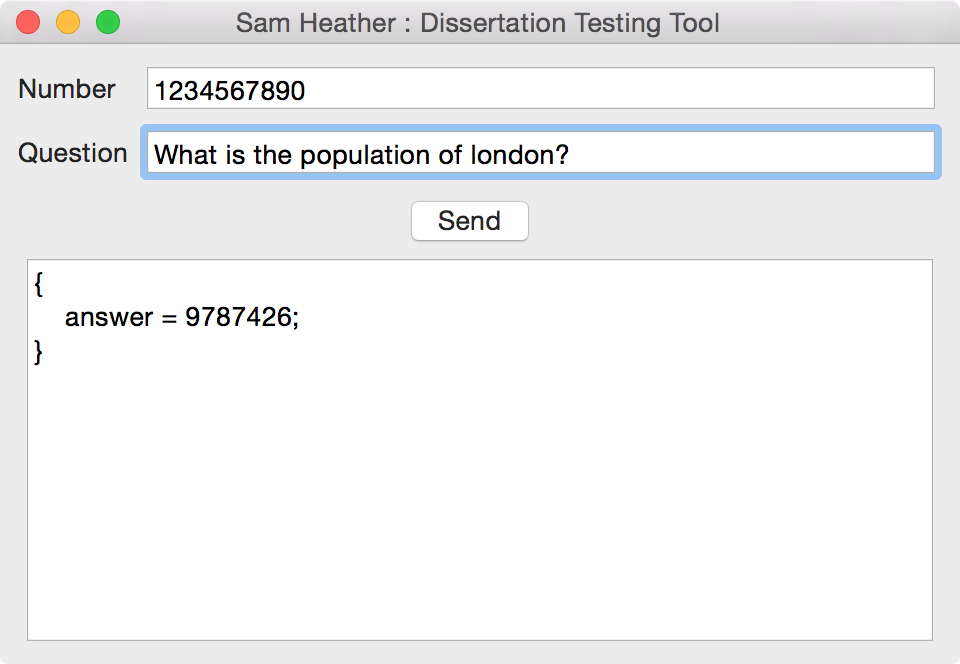
\includegraphics[width=300pt]{devClient}
    \caption{Development and testing client for Mac OS X showing a sample query}
    \label{fig:devClient}
\end{figure}

\section{Implementation and iteration of iOS app used in experimental evaluation}
\label{sec:implementationExperimentClient}
As described in section \ref{sec:evaluatingSuccess} an iOS app was created to act as a query interface for the server application for the experimental evaluation. This was written in Objective-C meaning it was trivial to port the implementation used in the testing client in section \ref{sec:implementationTestingClient}.

After running the dry run of the experiment three usability issues were identified resulting from the use of the iOS Simulator on the Mac platform: the on-screen keyboard remained visible covering text on some longer answers; the participant ID field at the top of the screen caused confusion with one dry run participant attempting to change the value; it was slow to clear the question field to send a new query. Also, both users would press \texttt{return} as opposed to clicking the \texttt{Go} button, which wouldn't send a question.

Fixes were made to the software before running the full experimental evaluation such as:
\begin{itemize}
  \item Questions are now sent both if either the \texttt{Go} button is tapped or the \texttt{return} button is pressed on the keyboard.
  \item When a query is sent, the on-screen keyboard is hidden as seen in Figure \ref{fig:experimentClientParis}. It can be brought back by tapping on the question field.
  \item When selecting the question field, all the text is selected by default making it easier to type a new query without spending time deleting the old text. A 'clear field' cross button which is standard on the iOS platform is also shown. This is shown in Figure \ref{fig:experimentClientPopulation}.
  \item The field to enter participant ID is hidden, as shown in \ref{fig:experimentClientParis}. This is now requested in a modal alert when the application starts: the ID is then entered by the researcher.
\end{itemize}

\begin{figure}[htb]
    \centering
    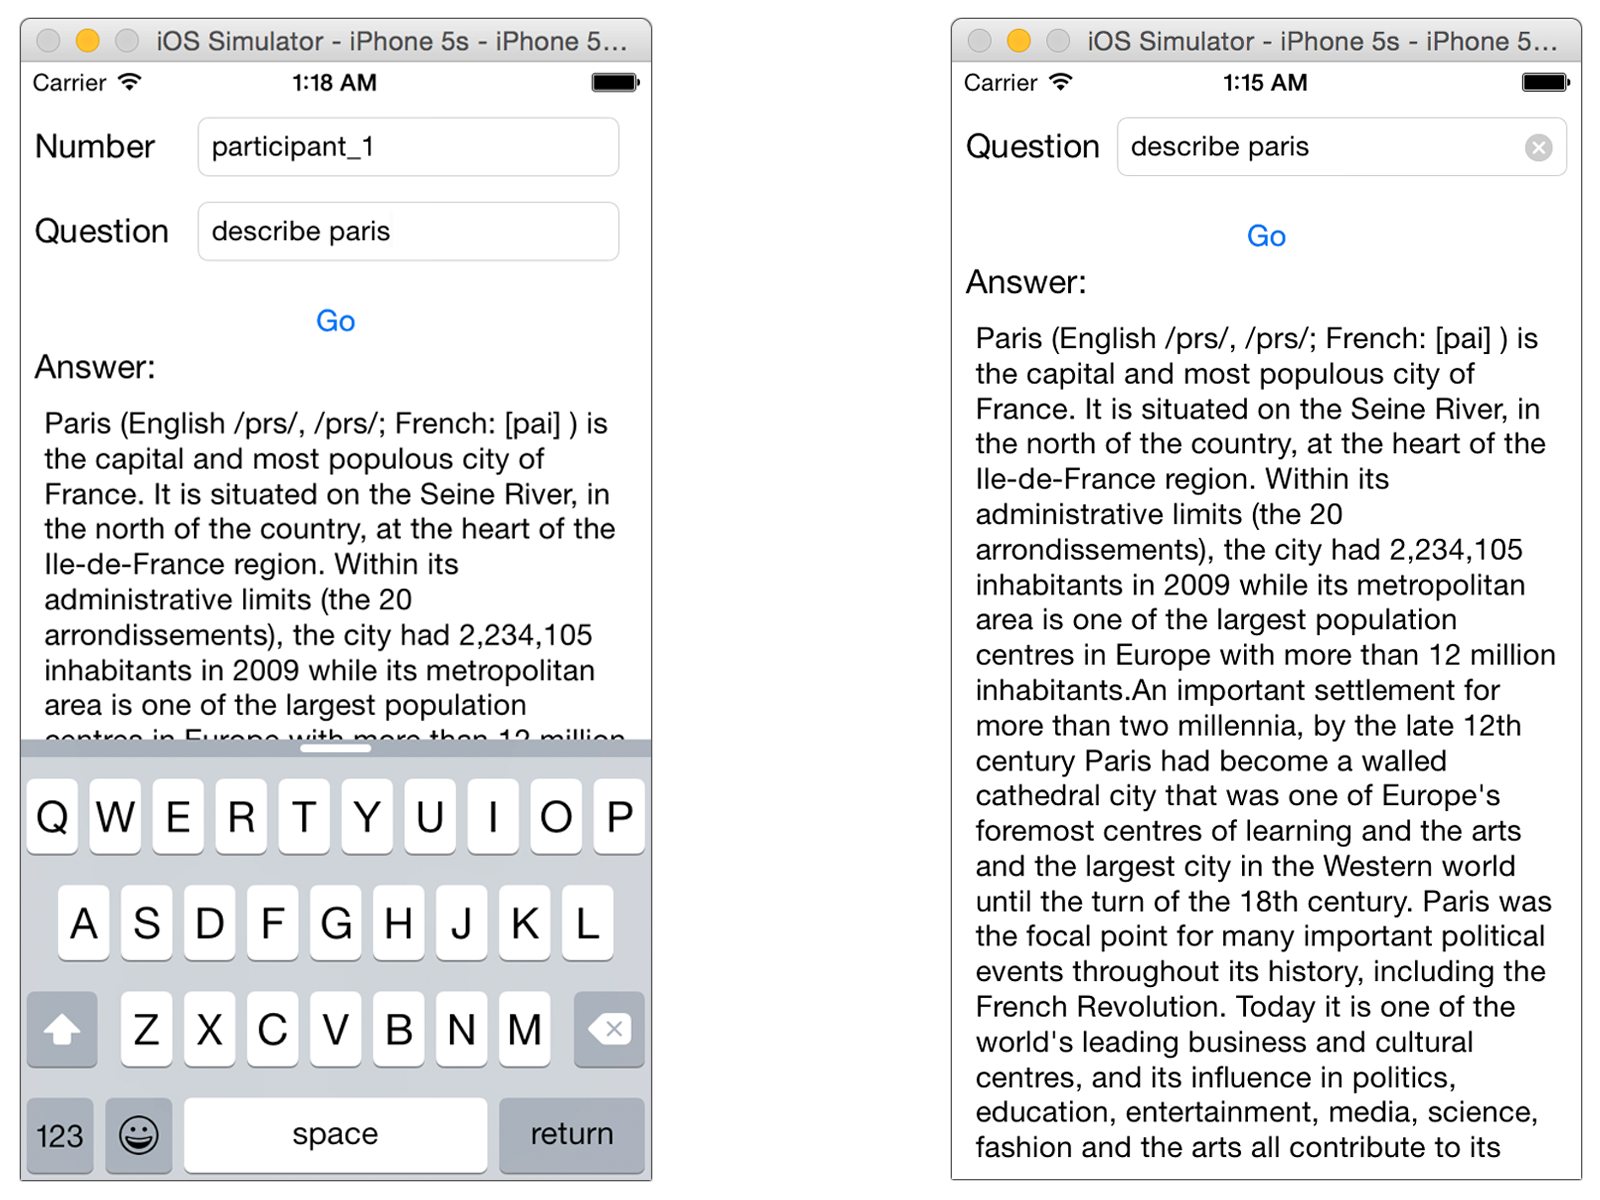
\includegraphics[width=\linewidth]{describe_paris}
    \caption{Left: Original application. Right: Revised application with keyboard hiding.}
    \label{fig:experimentClientParis}
\end{figure}

\begin{figure}[htb]
    \centering
    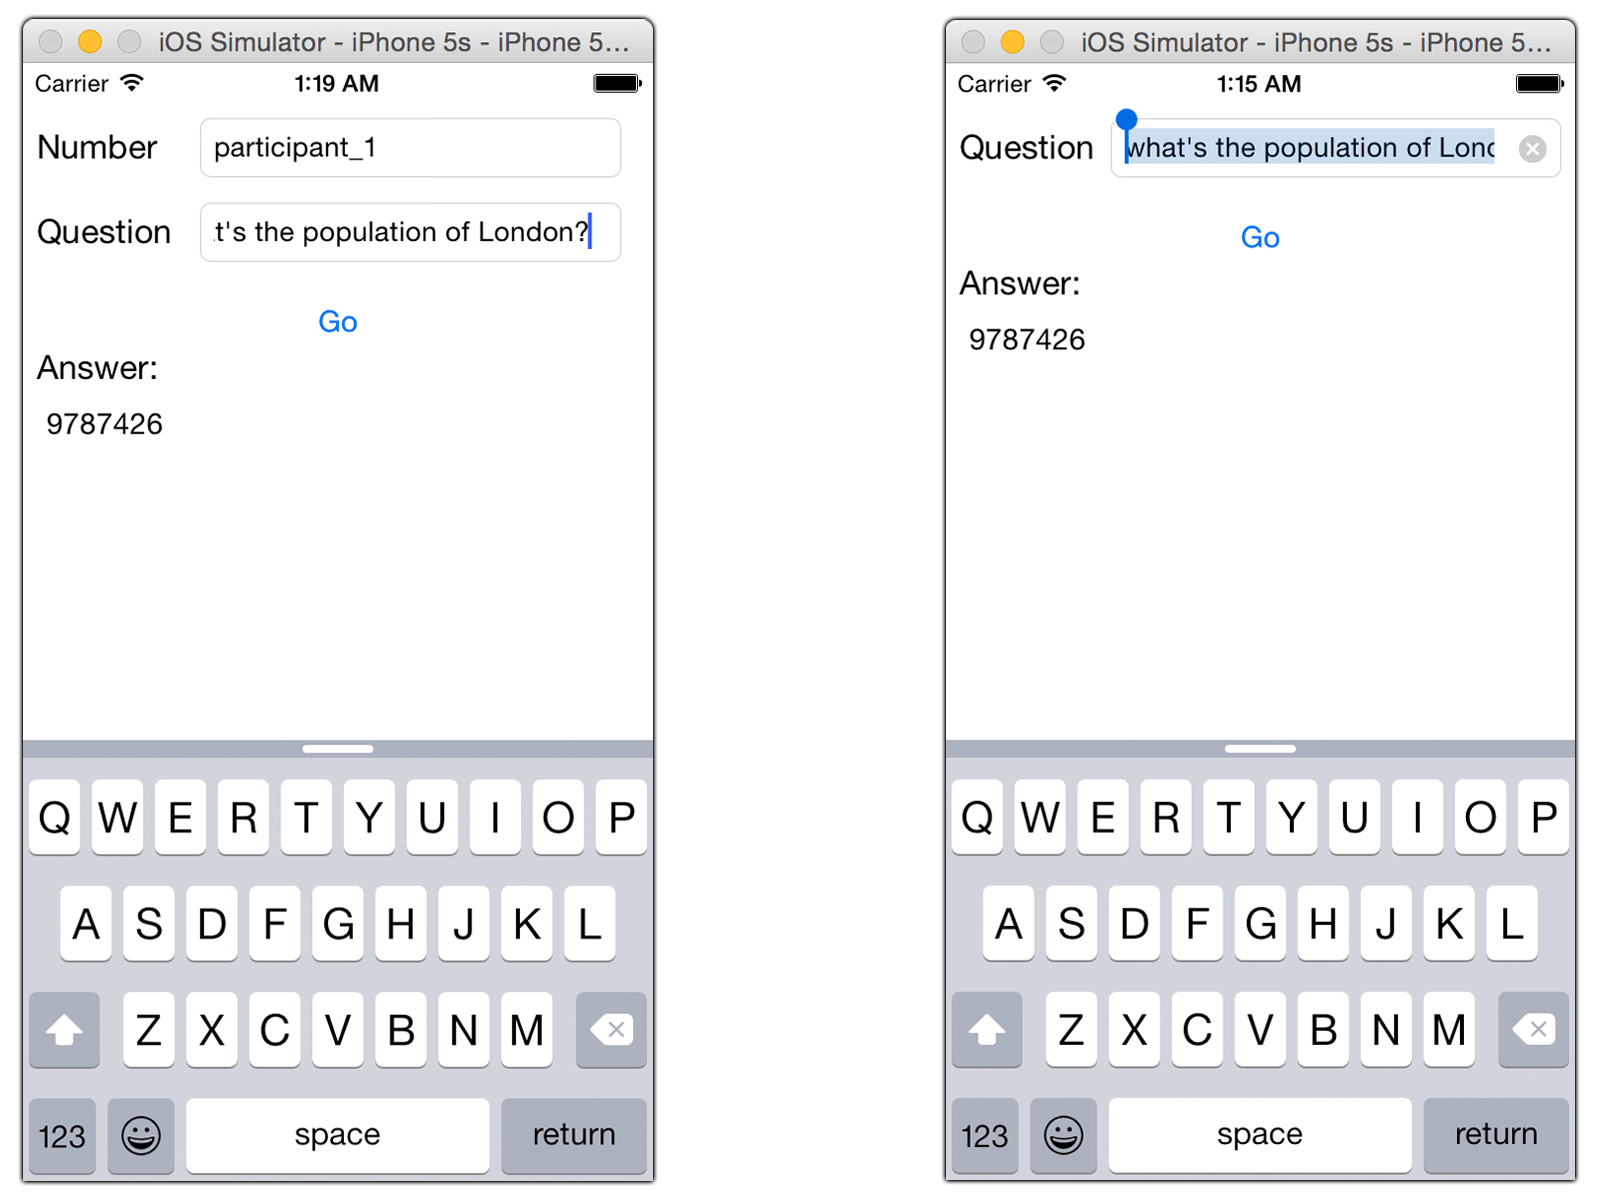
\includegraphics[width=\linewidth]{population}
    \caption{Left: Original application. Right: Revised application with hidden participant ID field and Question field with a clear button and auto-selection of text when it's tapped to bring the keyboard up.}
    \label{fig:experimentClientPopulation}
\end{figure}

\section{Adding Multi-Language Support}
\label{sec:addingMultilanguageSupport}
As described in section \ref{sec:planForSoftwareDevelopment} the software was initially intended to have support for multiple languages. Although this was not included in the software developed, the software has been constructed with an awareness of this potential future feature so that it can easily be added.
...%TODO Add with diagrams.

\section{Discussion of implementation and issues faced}
% TODO XXX - write this
% TODO - write about issues faced.
 - Tweaking the constants for best results
 - Excluding wikipedia due to dirty data
 
 \ref{sec:planForSoftwareDevelopment} - stuck to the iterative plan.
 
Key issues:

 - can't handle units
 
 - sometimes wikipedia attaches other garbage
 
 - can't do subjective stuff 'depth of the deepest ocean'
 
 - can't do properties that are stored deep within the ontology.
 
 - translation not done (here or extending this project?)

\newpage
\chapter{Results}
\label{sec:results}

In this chapter the results from the experiment will be discussed with information on the pool of participants used.

\section{Participants}
\label{sec:participants}

21 participants were sourced to take part in the experimental evaluation of this project. Participants were mainly sourced from the University of York however a small number did come from other locations such as Bristol when the researcher made an unrelated trip there.

Participants were heavily skewed towards young students: 17 participants identified as been aged 18-24 and 14 as students. Of the remaining participants, two were aged in the range 25-34 and the remaining two in the range 45-54.

Three of the non-student participants identified as been self-employed, one identified as been employed and one as retired. Additionally, two participants identified multiple occupations: one selected employed and self-employed, whilst another indicated self-employed and student.

All participants in the experiment were regular internet users with all participants identifying their typical Internet usage been 'multiple times per day' or greater. 7 participants selected 'multiple times per day' whilst 14 selected 'more than once per hour'.

\section{Results}
\label{sec:results}

In this section the results from the experiment are presented.

\subsection{Usefulness}
\label{subsec:resultsUsefulness}

The usefulness of the system is measured by questions 1 through 6, 13 and 14 in the questionnaire. The average of usefulness ratings was 3.51 (3.s.f.) with a standard deviation of 0.919. One standard deviation of the data from the mean (containing 68\% of the data points) put the usability of the system in the range 2.59 through 4.43.

\subsection{Usability}
\label{subsec:resultsUsability}

The usability of the system is measured by questions 7 through 12 in the questionnaire.  The average of usability ratings was 3.46 (3.s.f.) with a standard deviation of 0.810. One standard deviation of the data from the mean (containing 68\% of the data points) put the usability of the system in the range 2.65 through 4.27.

\subsection{Machine Learning}
\label{subsec:resultsMachineLearning}

A mean value of usefulness as rated by each participant was calculated using the values from questions 1 through 6, 13 and 14 and plotted. Linear regression was then carried out to identify whether a positive correlation existed showing that participants were indicating they would find the application more useful as more participants used it before them. The Correlation Coefficient for this dataset was 0.506.

A graph shoeing usefulness plotted against the participant number is shown in figure \ref{fig:usefulnessTrend} Using linear regression a line of best fit was added to the graph with the equation $y = 0.075 x + 2.68$.

\begin{figure}[htb] 
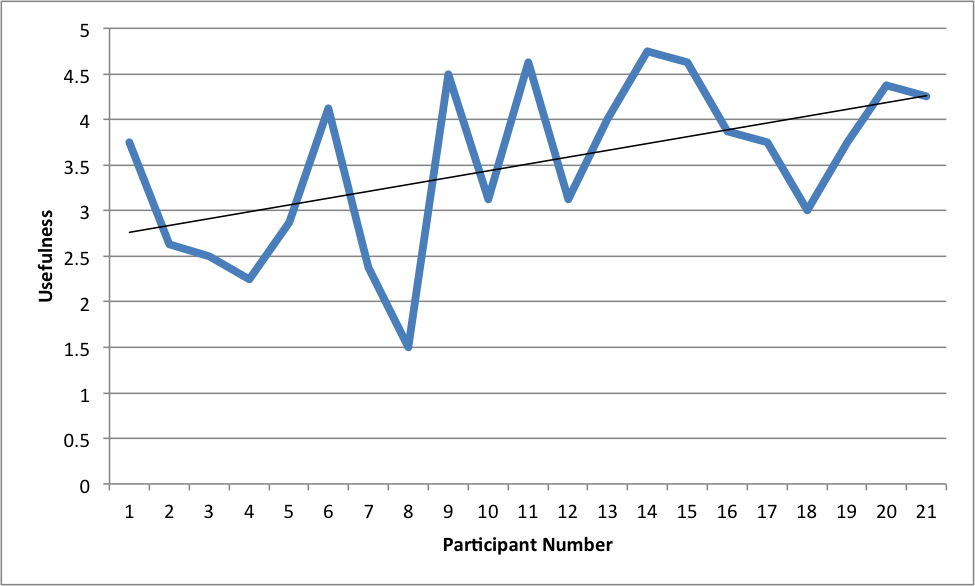
\includegraphics[width=\linewidth]{usefulnessTrend}
\caption{Graph showing Usefulness as rated by participants against participant ID with a trend line.}
\label{fig:usefulnessTrend}
\end{figure}

\subsection{Additional comments from participants}
\label{subsec:resultsComments}

No space was made on the questionnaire for participants to write additional comments or thoughts on the system, however two participants did make a comment at the end of their forms, both of which addressed a specific issue. These comments were:

\blockquote{I thought the detail generated from the answers to the describe questions were really detailed and informative, although displaying the units in other answers would have been helpful.} - Participant 14.

\blockquote{Answers with units would be helpful to understand values given as answers} - Participant 9.

These can't be included in any analysis due to not asking for a comment from all participants, but the issue will be discussed in the Discussion in section \ref{sec:discussion}.

\newpage
\chapter{Discussion}
\label{sec:discussion}

In this section the results from section \ref{sec:results} are analysed and discussed. The key piece of research been investigated is whether the application learns effectively, although the discussion will also look at the usefulness and usability results individually.

\section{Discussion of Results}
\label{sec:disResults}
In section \ref{sec:evaluatingSuccess} the success criteria for both usefulness and usability is defined as 'a significant positive average rating' for the relevant questions. Both the mean ratings and standard deviations for both the usefulness and usability questions were very similar - both show a slightly-above-neutral mean rating of the system, and the standard deviation shows the data is moderately distributed over the full range of possible ratings (it was not highly concentrated or well distributed).

Because of the spread of the results it is not all-together clear whether there is a significant positive view of the usefulness and the usability of the software. However, as the mean is above the neural point of \texttt{3} by 0.51 and 0.46 respectively (representing ~1/8th of the range of possible ratings) it is justified to state that the software was rated as having neutral or greater usefulness and usability. This does not fulfil the initial success criteria from section \ref{sec:evaluatingSuccess}, but still shows the software developed was not rated 'useless' and so has potential to become useful.

% TODO - come back and do a significance test on 'is it significant and high enough?'

%Learning
The results for showing the learning of the application, which was the key thing been measured, show that the application was successfully learning. As discussed in section \ref{sec:evaluatingSuccess}, the usefulness was evaluated according to a positive trend in feedback from participants as the number of participants who have used the application prior to them increases. A positive trend line can clearly be seen in the graph showing rated usefulness against the number of preceding participants. The correlation coefficient indicates that there is a moderate positive trend, which implies that the application was learning and its usefulness improving as more participants used it. This is therefore a success in the context of this project.

The graph showing rated usefulness against the number of preceding participants does show that the data collected is 'noisy' with a lot of variation in the ratings given by different participants. It is speculated that this was caused by the different levels of expectations that participants had. The questionnaire was worded to remind participants that they should rate the system in the context of them having no other access to the internet, but it is likely some participants considered this more than others whilst rating the application, sometimes making comparisons to other services from well-known consumer products that they have used.

It's noted that the participants were skewed towards a young student population with regular access to the internet. All participants identified as users who typically use the Internet multiple times daily and so some perhaps had difficulty imagining themselves working in the context of not having access to the Internet.

Also, as was mentioned in the Results in section \ref{sec:results}, two participants did note an issue on the questionnaire about units not been returned with the data, for example with questions about the \texttt{height} of a structure. Although this issue was noted before the experimental evaluation, the significance of not having units had not been fully considered and it was helpful to have this indicated by the participants.


\section{Data loss}
\label{sec:dataLoss}

It was initially planned to keep log files during the experiment containing the questions asked, answers provided and the ratings from a user. This would allow for the possibility of further analysis such as the identification of specific questions that caused users a problem or questions where the answer returned changed as more participants took part. However due to a bug where log files were over-written instead of having new entries appended to them, log files for participants up until participant number 14 were not stored. The seven remaining log files were too small a dataset to analyse, however some examples may be used in later chapters.

\newpage

\newpage
\chapter{Evaluation}
\label{sec:evaluation}

This Chapter aims to provide an evaluation on the experimental evaluation that was run and the software that was developed. The experiment will be evaluated based on the results, and the software will be compared to the original requirements in section \ref{sec:requirements}.

\section{Evaluation of Software Developed}
\label{sec:evalSoftwareDeveloped}

The success of the software developed according to the experimental evaluation has been discussed in the Discussion chapter in section \ref{sec:discussion}. However it's also important to check the software against the requirements originally proposed. The software has been compared to the User Requirements from section \ref{subsubsec:userRequirements} in table \ref{table:evalUserReqs}. In this table it is shown that all user requirements for the system were met apart from user requirement \ref{requirement:getFact} which is partially met. User requirement \ref{requirement:getFact} refers to the fact that units are not always returned with answers and this is a usefulness failure in the system. A proposal for future work to fix this is proposed in section \ref{sec:evalUnits}. The application meets all other user requirements fully.

The software is also compared against the non-functional requirements proposed in section \ref{subsubsec:systemRequirementsNonFunctional} in table \ref{table:evalNonFunctionalReqs}. In this table it is shown that the application meets all non-functional requirements except NF.2, which is that the application returns the correct answer for 90\% of queries. This requirement was marked as not met as the data that would have been used to evaluate it was lost, as described in section \ref{sec:dataLoss}. It was suggested that the ratings provided for application usefulness in the questionnaire would have been higher if this requirement was met.

% explain what can be done to improve this
% sumarise, only 2 requirements not fully met, acceptable.

TODO: explain what can be done to improve this; sumarise, only 2 requirements not fully met, acceptable.

\begin{table}[h]
\begin{tabular}{|p{0.4cm}|p{9.0cm}|p{4.0cm}|}
\hline
ID & Discussion                                                                                                                                                                                                                                                                                                                                                                                                                                & Conclusion                          \\ \hline
1  & Two types of questions were accepted: questions where a property was requested of a geographical entity; and questions where a user could ask the application to describe an entity.                                                                                                                                                                                                                                                      & This requirement was met.           \\ \hline
2  & Users were able to ask questions about a specific property, fact or statistic, however in some cases the units were not returned which reduced the usefulness of the answer. This occurred in a significant number of cases, such as whenever a measurement of an entity was requested, so the requirement wasn't fully met.                                                                                                              & This requirement was partially met. \\ \hline
3  & The Twilio service and API was used to create an SMS interface to the system.                                                                                                                                                                                                                                                                                                                                                             & This requirement was met.           \\ \hline
4  & Users were able to make queries quickly by entering them in natural language form, and a response was returned within a a few seconds.                                                                                                                                                                                                                                                                                                    & This requirement was met.           \\ \hline
5  & A ratings system was implemented to allow a user to give feedback on the last answer they received, which was subsequently used to improve the quality of future answers.                                                                                                                                                                                                                                                                 & This requirement was met.           \\ \hline
6  & Help and tutorial functionality was provided in the system and was available for users by simply sending a message with the world \texttt{help}. This was not tested during the experimental evaluation however, as a tutorial was given in the instructions for the experiment. Feedback from the experiment did show that users quickly learnt to use the system though, indicating that they were able to learn the system themselves. & This requirement was met.           \\ \hline
7  & A privacy protection system was implemented. Participants in the experiment were not made aware of this as the experiment focussed on answer quality, however they were comfortable with the privacy they had for their experimental data (explained on a consent form).                                                                                                                                                                  & This requirement was met.           \\ \hline
8  & Natural Language Processing was added to the application to allow users to make queries in natural English sentences. Users used this in the experimental evaluation and it was rated neutrally or above as part of the usability questions.                                                                                                                                                                                              & This requirement was met.           \\ \hline
\end{tabular}
\caption{Evaluation of User Requirements}
\label{table:evalUserReqs}
\end{table}

\begin{table}[h]
\begin{tabular}{|p{0.7cm}|p{9cm}|p{4.0cm}|}
\hline
ID   & Discussion                                                                                                                                                                                                                                                                                                                                     & Conclusion                    \\ \hline
NF.1 & The time from receiving a query to sending a response was typically under 10 seconds during development, which is less than the 20 second fit criterion.                                                                                                                                                                                       & This requirement was met.     \\ \hline
NF.2 & Due to the loss of log file data it is not possible to analyse the question logs to check against this criteria. However it is speculated that usefulness ratings from the experimental evaluation would have been higher than they were if 90\% of questions were answered correctly first time so it is assumed this requirement was not met. & This requirement was not met. \\ \hline
NF.3 & The ratings system implemented did prevent poor answers been returned after they were rated as such. Examples were given in section \ref{subsec:usingRatings}.                                                                                                                                                                                 & This requirement was met.     \\ \hline
NF.4 & The help information was not used during the experimental evaluation however users did not need further assistance when using the application beyond the instructions provided for the experiment, and the instructions provided were based on the instructions in the application.                                                            & This requirement was met.     \\ \hline
NF.5 & Participants used natural language to ask questions of the application during the experiment.                                                                                                                                                                                                                                                  & This requirement was met.     \\ \hline
\end{tabular}
\caption{Evaluation of Non-Functional Requirements}
\label{table:evalNonFunctionalReqs}
\end{table}

\section{Evaluation of Experimental Evaluation}
\label{sec:evalExperimentalEvaluation}

The experimental evaluation suffered from issues caused by the pool of participants used. As discussed the data was extremely noisy and it was speculated that this was caused by varying levels of expectation from participants. This could have been fixed by spending more time with each participant explaining the expectations they should have of the software and a typical situation in which it would be used. 

The participant pool contained 21 individuals and was extremely skewed towards students in the age range of 18-24 who used the internet multiple times per day. This is not representative of the range of possible users of the application developed, notably the personas developed in appendix \ref{sec:appendixPersonas} which were used to drive the user requirements.

Only 21 participants were used for the experimental evaluation, and each participant was asked to identify 16 pieces of information. The application learns more as each participant takes part and it would have been interesting to see if the trend of increasing ratings of usefulness continued with a larger number of participants. Time restrictions limited the number of data points that could be collected from each participant: with 16 pieces of information to identify the experiment took around 10 minutes during a test run. It would have been preferable to have more data points from asking participants to identify more information as this would perhaps have reduced the noise in the data due to a single poor result having less of a part of the whole experiment. Unfortunately this would have extended each run experiment making it more difficult to recruit participants without a remuneration for their time.

% TODO:     - more participants, does curve continue, get less noisy,
% TODO:     - more data

\newpage

\chapter{Extending this project}
\label{sec:extending}
{\bf Section not complete}
In this chapter solutions for some of the issues addressed in the evaluation will be presented as work that can be undertaken in the future to improve the software developed.

\section{Obtaining and presenting units for measurements}
\label{sec:evalUnits}
One of the major issues with the application developed is that units are not returned with all measurements. This is a direct result of the quality and inconsistent format of the data in the data sources. For some geographical entities units are stored in the field when the field type is a string, however in other entities the unit is stored in the key, for example \texttt{height\_m} is used to represent the height in metres. It should be possible to customise the processor for each data source in the source-specific module to handle this in the future.

\section{Improving the Natural Language Processing module}
\label{sec:evalNlp}
It was noticed both during development and informally during the experiments that the Natural Language Processing module isn't yet at the standard that a user expects. Although queries can be made in natural language, the structure of the question must be extremely simple. This is because of the way the property a user is requesting is identified, where additional unnecessary words in the query cause the process to fail. There were two example of this, one that arose during testing and one from the log files collected from the experimental evaluation. The first example was where the word \texttt{please} was added to a query, for example \texttt{How tall is the Eiffel Tower please?} which resulted in the application searching for the property \texttt{tall please}. The second example from the experimental evaluation occurred when a user was asked to identify the \texttt{currency that we use in England}. A typical query was \texttt{What currency is used in England?}, which resulted in the application searching for the property \texttt{currency used} instead of just \texttt{currency}. This also resulted in the application failing.

In future work the natural language processing module can be improved to cope better with noise, perhaps through the use of a more complex third-party library.

\section{Expanding the range of subjects from Geography}
\label{sec:evalExpandingSubjects}
Geography was selected as the topic area to perform research on in this project because it was a topic with few ethical issues, as discussed in the introduction in section \ref{sec:introAimsOfThisProject}. If the ethical issues could be addressed and resolved, interesting future work includes expanding this application to work with Wikipedia resources from a larger number of subject areas. There would also be some engineering issues: the current software is dependent on knowing that a query is about a geographical entity. As the range of possible entity types expanded there will be issues in identifying the specific entity that a user is inquiring about if a query contains multiple entities or concepts.

\section{Add support for multiple languages}
\label{sec:evalMultipleLanguages}
This has been discussed in section \ref{sec:addingMultilanguageSupport} in the implementation as detail was given as to where it would fit into the application. 

\section{Using SPARQL to perform complex queries in DBPedia}
\label{sec:evalSparql}
One area where significant progress can be made in the software is with queries to the DBPedia ontology. In section \ref{subsec:dbpediaOntology} the available interfaces to DBPedia are discussed and the issues with creating SPARQL queries presented. The main issue is one of software complexity: taking a query in natural language form and then constructing a formal Ontology query is difficult as terms in the query have to be matched to classes in the Ontology. However if this were to be achieved the results that the Ontology could return would be significant of significantly higher quality as data that is abstracted into linked objects could be retrieved. An example of this is the query \texttt{Who is the mayor of London?}. The object \texttt{London} in the DBPedia Ontology does not have a field \texttt{Mayor}, but instead a pointer to another object called \texttt{Mayor\_of\_London} which contains the data requested. This was beyond the scope of the original project due to the time constraints, as this will not be a quick feature to implement.

\newpage

\chapter{Conclusion}
\label{sec:conclusion}
Currently been worked on in Google Docs...

\newpage

\bibliographystyle{IEEEtran}
\bibliography{IEEEabrv,mybib}

\appendix
\part{Appendices}

\newpage
\chapter{Personas}
\label{sec:appendixPersonas}
\section{Nanjala}
\subsection{Demographics and Profile}
\begin{itemize}
  \item Female, aged 15
  \item Living in the village of Amuria, Uganda, 300km from the capital Kampala.  Internet access is difficult and expensive to obtain in Amuria, though there is good mobile network coverage.
  \item Currently in general education at her village school.
  \item Nanjala is curious and wants to be able to ask questions and retrieve and read more information at her own leisure.  She prefers to be told about something than to learn facts.
\end{itemize}
\subsection{Average Day}
In a typical day, Nanjala will rise early to help her family with housework chores, before she prepares for school.  Nanjala wants to become a teacher.  At school, she studies Science, Maths and Geography, and works hard for her classes and on her homework.  Nanjala's school has a small library and a large body of students, meaning that books are often unavailable when Nanjala would like to look something up.  This increases the amount of time that her homework takes, and can even result in her not having access to information when she goes home.

\newpage
\section{Cedric}
\subsection{Demographics and Profile}
\begin{itemize}
  \item Male, aged 27
  \item Lives in Zurich, Switzerland, and goes on regular hiking trips, from 3-4 day trips around Europe to longer trips to the South American Andes and southern Asia.
  \item Works in a service role in the city and so has little disposable income to spend on guide books for the many places he visits.
  \item Cedric is a competent albeit not professional hiker, often going off-track and summiting 'difficult' peaks or reaching famous camping grounds.  He likes to be spontaneous, only deciding which peaks he will attempt when he arrives.
  \item Cedric is very conscientious and wants to contribute his own knowledge to the world, especially to projects that help him.
  \item Cedric values his privacy is concerned about how much information he gives out online.
\end{itemize}
\subsection{Average European Trip}
A typical trip will involve an intercity train from the Zurich Hauptbahnhof (the main station) to the city closest to the range Cedric will be hiking.  He takes the train because it tends to be cheaper than flights.  Once in the area, Cedric will take local trains and buses to get into the mountain ranges.  There, he will use the local hiking trail network signs and conversations with the locals to select a peak or route.  Once Cedric has got moving and is reaching higher ground, he uses a combination of his view and the signage to identify other peaks that he would like to wander around.  

Cedric takes a non-smart phone with him because a) the battery life on his smart phone is not long enough for his whole trip, whereas his non-smart phone lasts a week at a time, and b) his smart phone would not be useful anyway, since the internet is so intermittent.  He still wishes he could get information such as whether there are maintained routes on the slopes of a given peak or the height of a peak that he sees without having to phone friends back in the city.
\newpage

\chapter{Sample Consent Form}
\label{sec:appendixConsentForm}
\newpage

\section*{System to access knowledge using Machine Learning and SMS - Usability and Usefulness Study}
{\parindent0pt
\subsection*{Informed Consent - Introduction}
This study aims to investigate the usability and usefulness of a system developed to provide access to knowledge using machine learning and SMS.  The system aims to provide high quality answers to questions asked of it, where the questions relate to either a description or property of a geographical entity (for example a city, river or mountain).  The system aims to learn where mistakes have been made and improve by receiving feedback from the user on the previous answer.  

\subsection*{Form: please complete this section before the study.}
I, \textunderscore\textunderscore\textunderscore\textunderscore\textunderscore\textunderscore\textunderscore\textunderscore\textunderscore\textunderscore\textunderscore\textunderscore\textunderscore\textunderscore\textunderscore\textunderscore\textunderscore\textunderscore\textunderscore\textunderscore\textunderscore\textunderscore\textunderscore\textunderscore\textunderscore\textunderscore\textunderscore\textunderscore\textunderscore\textunderscore\textunderscore\textunderscore\textunderscore\textunderscore\textunderscore\textunderscore\textunderscore\textunderscore\textunderscore\textunderscore\textunderscore\textunderscore, agree to participate in this study.  I have been briefed on and understand the purpose and goals of the project.

I understand that information will be collected from me during this study in the form of my answers to a questionnaire.  Additionally, I understand that my interactions with the application will be recorded, specifically the questions I ask, answers returned and my quality ratings of answer. I understand that this information will be treated confidentially and only Sam Heather and the project supervisor (Lilian Blot) will have access to the original data in its original format.  When the information is processed, shared, described or interpreted I will not be personally identified.

I understand that I can withdraw from the study at any point without giving a reason.

Date: \textunderscore\textunderscore\textunderscore\textunderscore\textunderscore\textunderscore\textunderscore\textunderscore\textunderscore\textunderscore\textunderscore\textunderscore\textunderscore\textunderscore\textunderscore\textunderscore\textunderscore\textunderscore\textunderscore\textunderscore\textunderscore
Signature: \textunderscore\textunderscore\textunderscore\textunderscore\textunderscore\textunderscore\textunderscore\textunderscore\textunderscore\textunderscore\textunderscore\textunderscore\textunderscore\textunderscore\textunderscore\textunderscore\textunderscore\textunderscore\textunderscore\textunderscore\textunderscore

{\bf Researcher's contact details:} Sam Heather, sam@heather.sh

{\bf Supervisor's contact details:} Lilian Blot, lilian.blot@york.ac.uk

\pagebreak

\subsection*{Post experiment consent form - please complete this section after the study.}
$\square$ I have been suitably debriefed about the system and my performance.

$\square$ I understand I can withdraw my data from the study at any time.

$\square$ I have not been forced to take part in this study.

$\square$ The Researcher has treated me with respect and answered all of my questions.

\vspace{10 mm}

For the researcher: Participant ID: \textunderscore\textunderscore\textunderscore\textunderscore\textunderscore

}

\chapter{Experimental Evaluation Instruction Sheet}
\label{sec:appendixExperimentalInstructions}
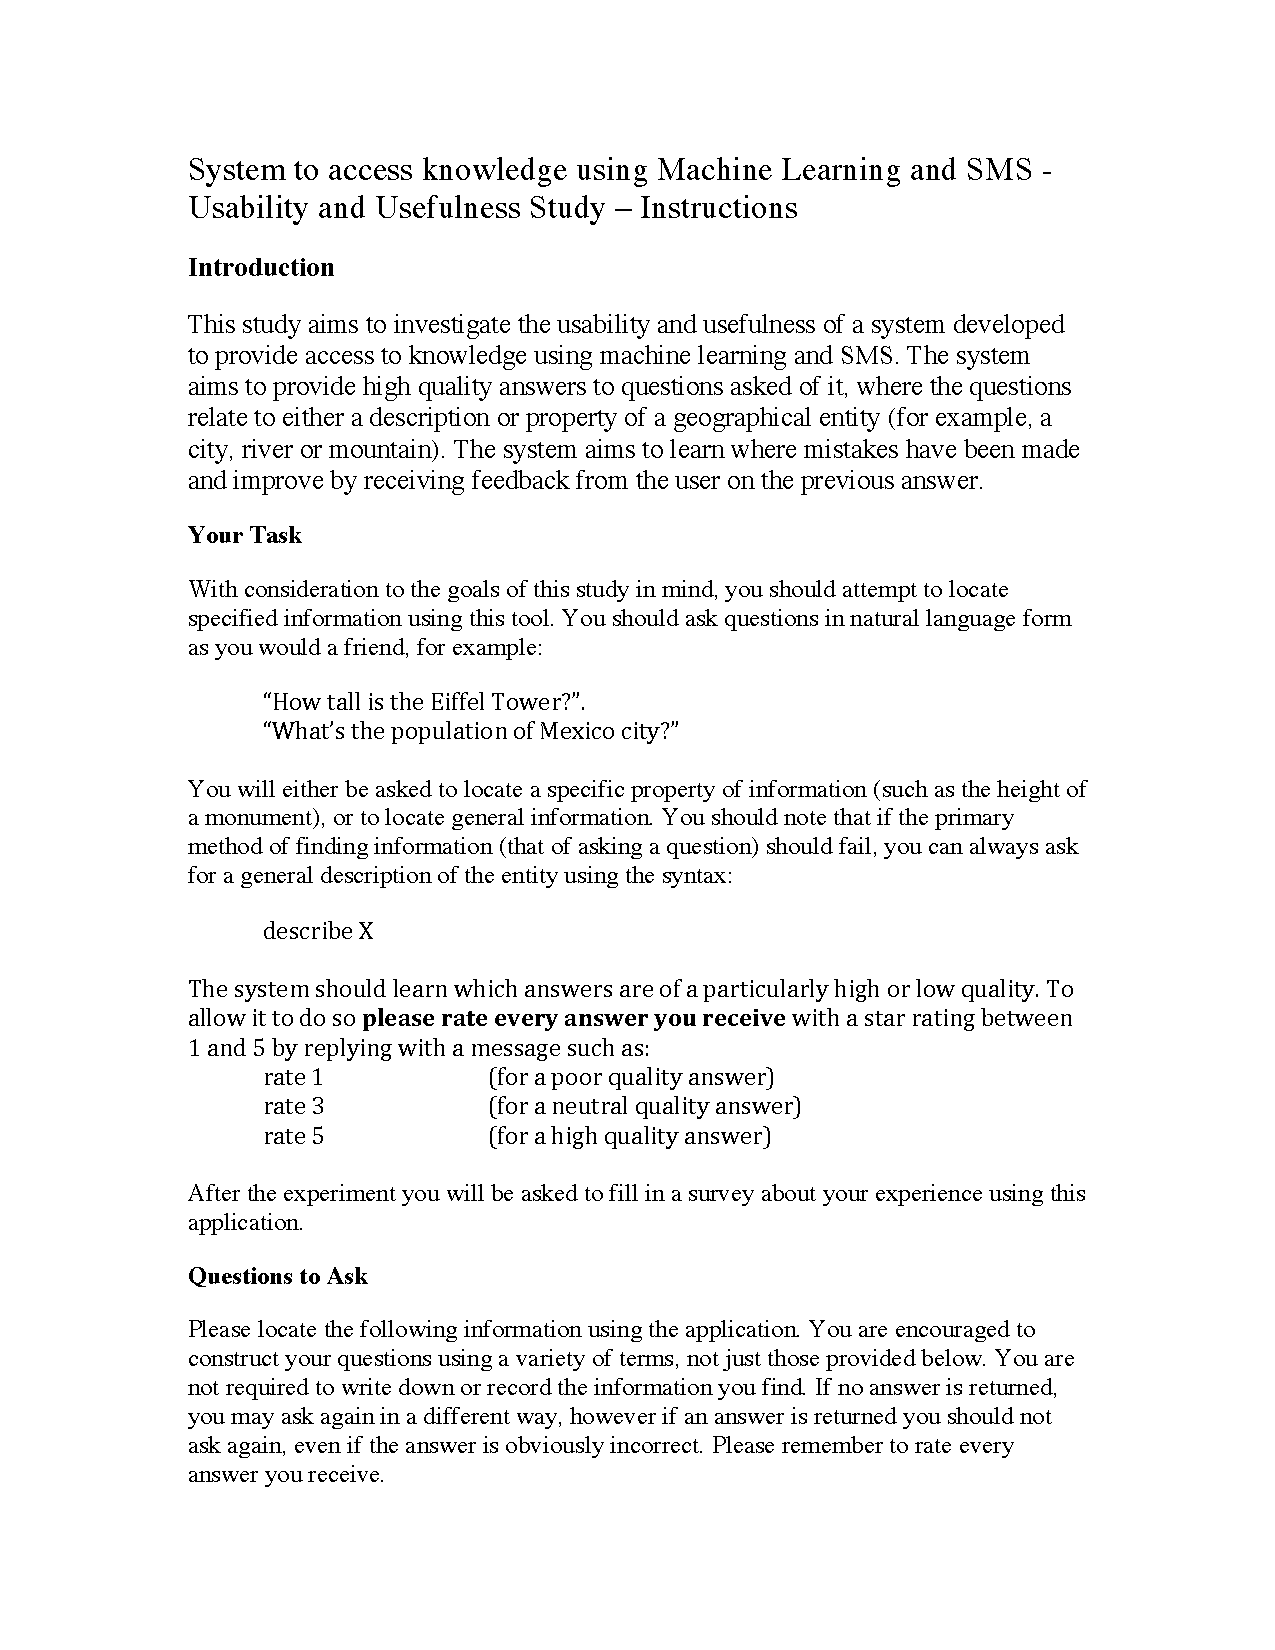
\includepdf[pages={1,2}]{Experiment_Instructions.pdf}

\newpage
\chapter{Sample Questionnaire}
\label{sec:appendixQuestionnaire}
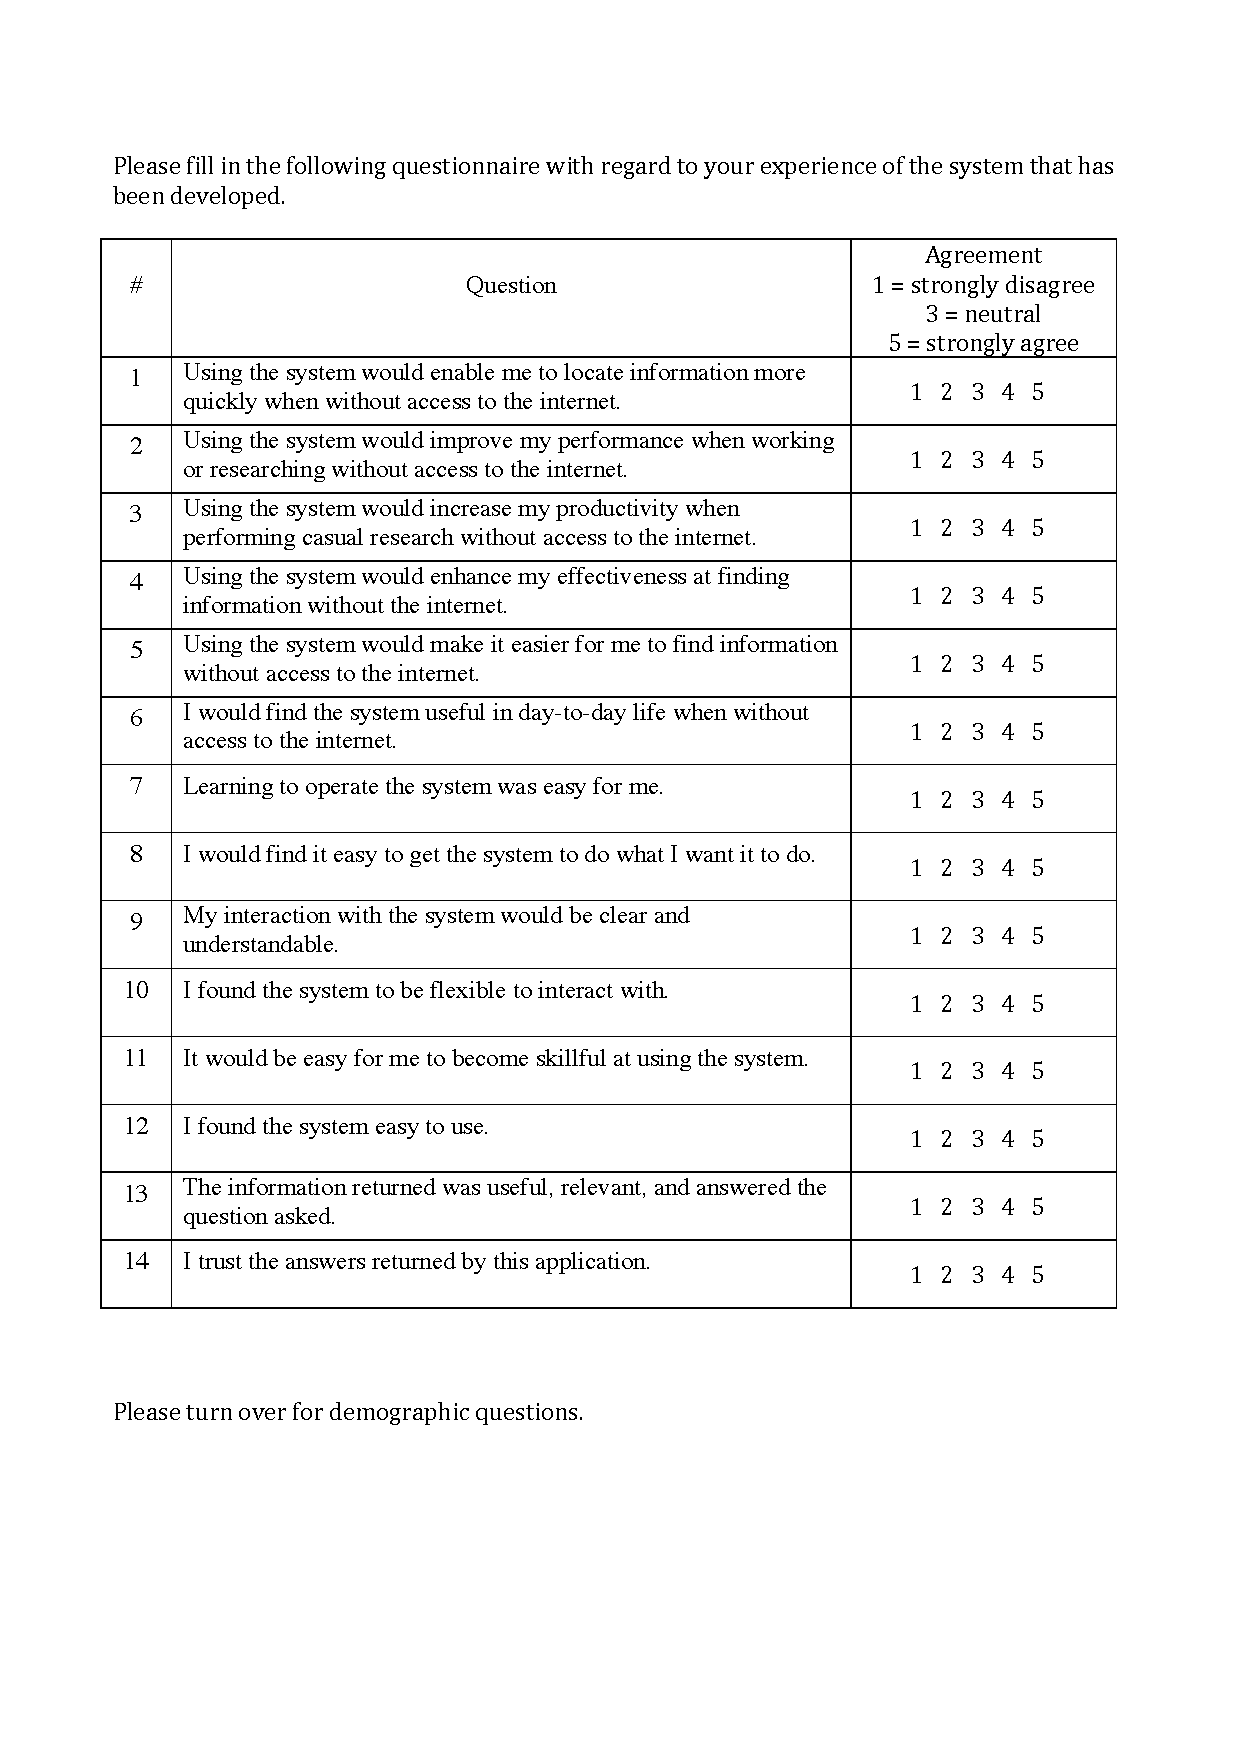
\includepdf[pages={1,2}]{Questionnaire_3.pdf}



\end{document}  %End of document.



















